\documentclass[journal]{IEEEtran} % use the `journal` option for ITherm conference style
\IEEEoverridecommandlockouts
% The preceding line is only needed to identify funding in the first footnote. If that is unneeded, please comment it out.

\usepackage{hyperref}
\usepackage{cite}
\usepackage{amsmath,amssymb,amsfonts}
\usepackage{algorithmic}
\usepackage{graphicx}
\usepackage{textcomp}
\usepackage{xcolor}
\usepackage{flushend}
\usepackage{graphicx} % To include images
\usepackage{float} % To use [H] for figure placement
\graphicspath{img}

\def\BibTeX{{\rm B\kern-.05em{\sc i\kern-.025em b}\kern-.08em
    T\kern-.1667em\lower.7ex\hbox{E}\kern-.125emX}}

\begin{document}

\title{Enhancing Spectrum Sensing For 5G and LTE\\ With Improved U-Net Architecture
\thanks{Corresponding author: Thien Huynh-The (thienht@hcmute.edu.vn)}}
\author{%%%% author names
    \IEEEauthorblockN{Huan Nguyen-Duy}~and \IEEEauthorblockN{Thien Huynh-The}% delete this line if not needed
    \\%%%% author affiliations
    \IEEEauthorblockA{Department of Computer and Communications Engineering}\\
    {Ho Chi Minh City University of Technology and Education, Ho Chi Minh City, $70000$, Vietnam}\\% first affiliation
    %%%% corresponding author contact details
    \IEEEauthorblockA{Email: huan$2931$@gmail.com, thienht@hcmute.edu.vn} \\
    % \IEEEauthorblockA{thienht@hcmute.edu.vn}
}
\maketitle

\begin{abstract}
Spectrum sensing for wireless communication plays a crucial role in next-generation networks, allowing devices to identify and accommodate the demand for wireless connectivity. In this paper, we address challenges in spectrum sensing and introduce an innovative deep network, namely Spectrum Sensing Network (SpecSenseNet) for over-the-air communication sensing. We propose an architecture derived from U-Net, integrating state-of-the-art approaches to enhance sensing performance. These approaches include depth-wise separable convolution, recurrent residual blocks, and Atrous Spatial Pyramid Pooling. They are designed to reduce the network's size while maintaining high prediction performance. Consequently, our design reduces effectively the number of parameter counts by $75.1\%$ compared to U-Net. In terms of evaluation, we generate a synthetic signal dataset containing two primary signal types, such as fifth-generation new radio (5G NR) and long-term evolution (LTE) adapted to various levels of additive noise in the range of $\left [ 0,30 \right ]$ dB. Regarding simulation results, our proposed network achieves impressive results, demonstrating high performance for spectrum sensing while maintaining excellent precision and significantly reducing the network's size. Our implementation and pre-trained model are available on
\href{https://github.com/Winxkin/Spectrum_sensing_base_on_Deep_learning.git}{Github}.
\end{abstract}

\begin{IEEEkeywords}
    spectrum sensing network (SpecSenseNet), spectrum sensing, 5G new radio (5G NR), long-term evolution (LTE), Unet, semantic image segmentation, signal processing.
\end{IEEEkeywords}

\section{Introduction}
\subsection{Spectrum sensing}
Spectrum sensing refers as identifying the availability and non-availability of wireless communication networks or radio networks in particular frequency bands. When a traditional frequency allocation scheme cannot provide high data rate demand constantly, it leads to waste spectrum resources. These resources can be allocated for others in need, such fifth generation new radio or long-term evolution simultaneously. Therefore, spectrum sensing for 5G NR and LTE has become a main topic currently presenting many challenges, focusing on performance enhancement of monitoring and managing limited spectrum resources effectively. The Fig.~\ref{fig1} shows an overview of spectrum sensing for 5G and LTE applications and services.

\begin{figure}[!ht]
    \centering
    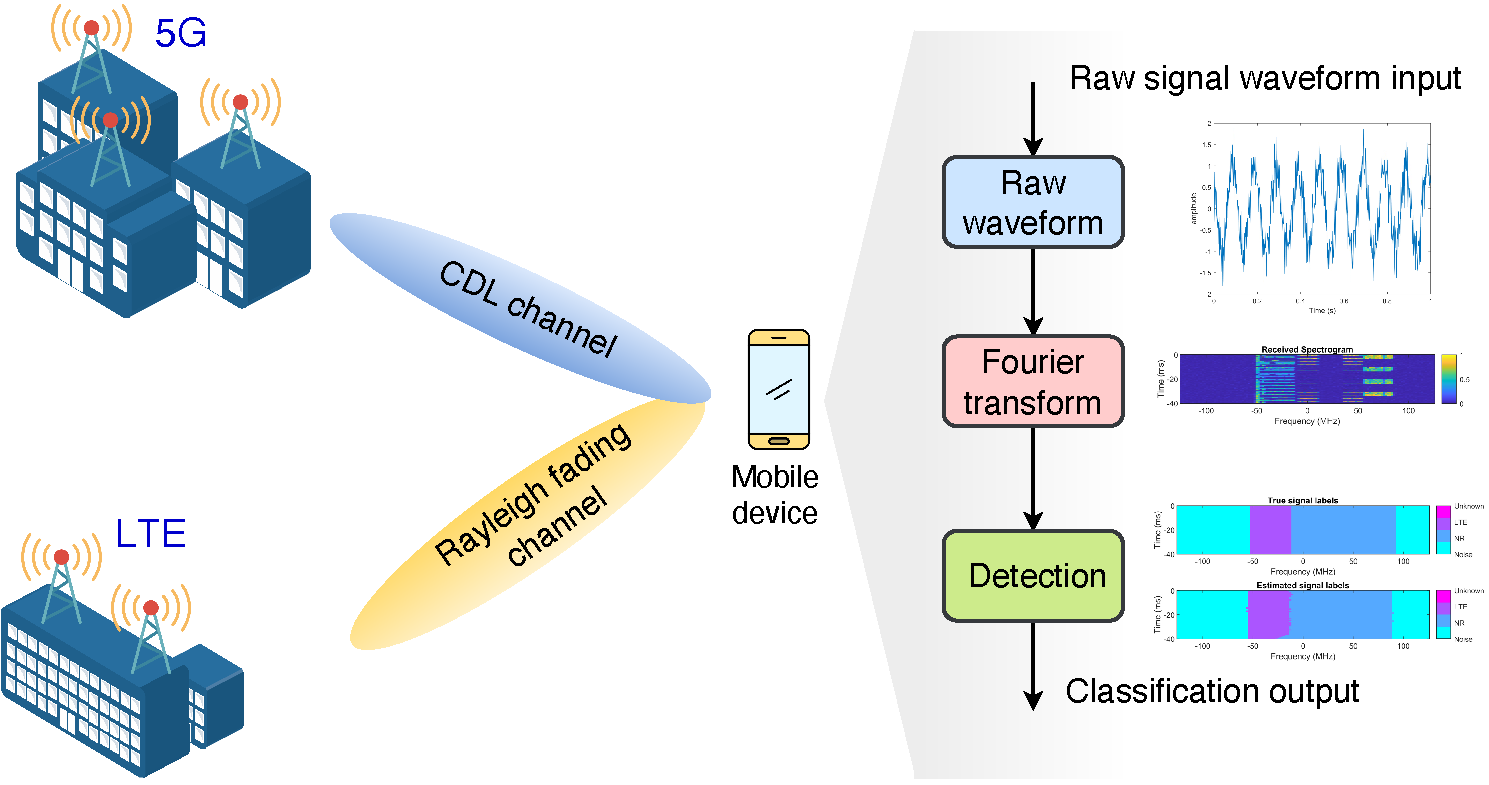
\includegraphics[width=0.45\textwidth]{img/Design-Overview.pdf}
    \caption{An overview of spectrum sensing for 5G and LTE.}
    \label{fig1}
\end{figure}

In the past, numerous sensing techniques have been introduced that utilize sensing algorithms, multi-dimensional spectrum sensing, channel estimation, and cooperative sensing. However, spectrum sensing faces a significant challenge in hardware requirements. It demands high sampling rates, high-resolution analog-to-digital converters with large dynamic ranges, and high-performance processors~\cite{YucekSpectrumSensing}. Cognitive wireless communication can be categorized based on sensing duration and frequency~\cite{kumar2024analysis}. However, this method involves a trade-off between performance and the complexity of sensing algorithms. Since their introduction, researchers have focused on improving spectrum sensing to address various challenges and introduce innovative solutions to increase accuracy and performance in cognitive wireless communication networks. Prominent surveys on this topic are provided in~\cite{ali2016advances, liyanaarachchi2021optimized}, where research directions and machine learning-based solutions for intelligent spectrum sensing are comprehensively investigated and discussed.



\subsection{Related work}

In recent years, significant research efforts have been directed towards enhancing spectrum sensing performance in cognitive wireless communication and radio networks. Several approaches have emerged, each with its own advantages and limitations. Energy detector-based sensing is a common method due to its low computational and implementation complexity. Waveform-based sensing offers improved sensing performance, while cyclostationarity-based sensing focuses on detecting and matching filtering transmissions from primary users.
However, traditional methods often present lower accuracy in spectrum sensing, especially in real-world environments with noise and channel impairments.
Deep learning (DL) approaches have also emerged as innovative solutions to improve spectrum sensing performance. In~\cite{huynh2024improved}, a  high-performance deep model with an convolutional neural networks (CNN) architecture was developed for improved waveform classification. Recently, the work in~\cite{huynhthe2023intelligence} introduced a novel DL architecture specifically designed to enhance the spectrum sensing prediction ratio for 5G and LTE signals. Other researchers have explored using DeepLabv3+~\cite{nguyen2023accurate} and DetectNet~\cite{gao2019deep} to increase the accuracy of spectrum sensing.
While deep models often achieve higher accuracy compared to conventional spectrum sensing approaches, there is still room for improvement in spectrum identification, particularly when dealing with noise and channel impairments.

\begin{figure}[!t]
    \centering
    \footnotesize
    \begin{tabular}{ccc}
        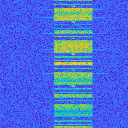
\includegraphics[width=0.13\textwidth]{img/LTE_frame_0.png}  & 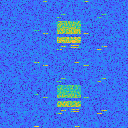
\includegraphics[width=0.13\textwidth]{img/NR_frame_1506.png} &
        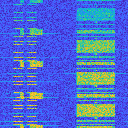
\includegraphics[width=0.13\textwidth]
        {img/LTE_NR_frame_0.png} 
        \\
        (a) & (b) & (c)
    \end{tabular}
    \caption{Spectrogram of received signals: (a) LTE, (b) 5G NR, (c) overlapping 5G NR and LTE}
    \label{fig2}
\end{figure}

\subsection{Contribution}
In this work, we leverage DL approaches to tackle sensing tasks and propose an innovative U-Net-based deep network architecture, called Spectrum Sensing Network (SpecSenseNet), which significantly reduces the network's size while enhancing sensing performance for 5G and LTE signals. 
Notably U-Net is a fully convolutional network well known for its effectiveness in semantic image segmentation, it is designed with a parallel encoder and decoder paths and connected together by skip connection wires~\cite{ronneberger2015u}. Recently, U-Net++ and other variant models\cite{zhou2019unet++} have shown notable improvements of segmentation accuracy; however, these models consume significant memory and computational resources. 
As a result, they are not suitable for resource-limited devices. 
To address this limitation, we present SpecSenseNet. This architecture incorporates depth-wise separable convolutions~\cite{CholletXception} and recurrent residual convolutions~\cite{AlomNuclei, he2016deep, aghalari2021brain} within the encoder and decoder paths, replacing standard U-Net blocks. These modifications effectively reduce the network's size without sacrificing segmentation accuracy. Additionally, Atrous Pyramid Spatial Pooling modules are integrated between the encoder and decoder paths to enhance the learning of relevant features at multiple scales~\cite{ChenAtrous}.
In summary, we make the following two main contributions:
\begin{itemize}
\item Addressing spectrum sensing for 5G and LTE problems and utilizing DL approaches to tackle spectrum sensing.
\item Introducing an innovative SpecSenseNet architecture based on U-Net that reduces significant network complexity in terms of the number of trainable parameters and maintains sensing performance for 5G and LTE signals.
\end{itemize}


\section{Methodology}
\subsection{Signal model}
Nowadays, over-the-air communication systems have a vital role in diverse scenarios and applications \cite{lin20215g}. This work mainly considers about 5G NR and LTE communication systems. In practical terms, received signals (called RX signal) from different sources can be defined as follows:
\begin{equation}
    {y(t) = x(t) \ast h(t) + n(t)},
    \label{eq:rxsig}
\end{equation}
where ${y(t)}$ denotes for the RX signal, ${x(t)}$ is the transmitted signal (called TX signal),  ${h(t)}$ is the channel response, and ${n(t)}$ refers to additive white Gaussian noise (AWGN).

% \begin{equation}
%     {E = \sum_{f = f_{\text{min}}}^{f_{\text{max}}} \left| Y(\tau, w) \right|^2}.
%     \label{eq:energy}
% \end{equation}


% \footnotetext[1]{ the operator * represents for convolution operation}

Short-time Fourier transform (STFT) is a widely used signal processing technique to analyze the frequency content of a signal over time. The RX signal (\ref{eq:rxsig}) can be presented in the frequency domain by STFT that is defined as follows:
\begin{equation}
    {Y(\tau, w) = \int_{-\infty}^{\infty} y(t) \cdot w(t - \tau) \cdot e^{-j2\pi ft} \, dt},
    \label{eq:spectrogram}
\end{equation}
where ${Y(\tau, w)}$ represents the spectrogram of the RX signal at frequency ${f}$ and time ${t}$, ${y(t)}$ is the input RX signal, and ${w(t - \tau)}$ denotes the window function used for segmenting the signal into short frames. 
Furthermore, the energy density of signal models is illustrated by 
\begin{equation}
    {E = \sum_{f = f_{\min} }^{f_{\max}} \left| Y(\tau, w) \right|^2},
    \label{eq:energy}
\end{equation}
where $E$ denotes the energy density in the range of frequency ${\left [ f_{\min}, f_{\max} \right ]}$.
Some spectrogram images obtained by STFT are illustrated in Fig.~\ref{fig2}, which present the spectrograms of 5G NR, LTE, and overlapping 5G and LTE. 
Clearly, with traditional spectrum sensing approaches, it is challenging to accurately discriminate the spectrum regions of these overlapped signals.



\subsection{SpecSenseNet: A robust and cost-efficient deep network}
In this section, we present the detailed architecture of the proposed Spectrum Sensing Network (SpecSenseNet) in Fig.~\ref{fig4}. This network is designed as a robust and cost-efficient convolution network based on U-Net architecture \cite{ronneberger2015u} for learning spectral signal patterns during the training state and identifying the waveform of received signals automatically in the prediction state. In general, SpecSenseNet exhibits a harmonious symmetry between its encoder and decoder paths, with each path interconnected by skip connection wires. It employs pooling operators to reduce the resolution of the input in the encoder path and upsampling operators to increase the resolution of the output in the decoder path. To effectively reduce the network's size while maintaining the prediction accuracy, we primarily employ three approaches: depth-wise separable convolution (DSC) \cite{CholletXception}, recurrent residual block (RRB)~\cite{aghalari2021brain, he2016deep}, and Atrous Spatial Pyramid Pooling (ASPP) \cite{ChenAtrous}. These approaches are instrumental in preserving accuracy while significantly decreasing the network's size. 

In particular, DSC \cite{CholletXception} is utilized as a convolution operator to replace for a regular convolution in the U-net architecture design \cite{ronneberger2015u}. DSC cooperatively employs depth-wise convolution and point-wise convolution to reduce significantly the size of network. The output of DSC $F_\text{out}^\text{DSC}$ can be expressed as follows:
\begin{equation}
    \mathrm{F}_\text{out}^\text{DSC} = \mathrm{relu}(\mathrm{pconv}(\mathrm{bn}(\mathrm{dwconv}(\mathrm{F}_\text{in}^\text{DSC})))),
    \label{eq:Fdsc}
\end{equation}
where $\mathrm{F}_\text{in}^\text{DSC}$ is the input of the preceding DSC, $\mathrm{dwconv}$ represents the depth-wise convolution, following by a batch normalization ($\mathrm{bn}$), a point-wise convolution ($\mathrm{pconv}$), and a ReLU activation function ($\mathrm{relu}$).

\begin{figure}[!t]
    \centering
    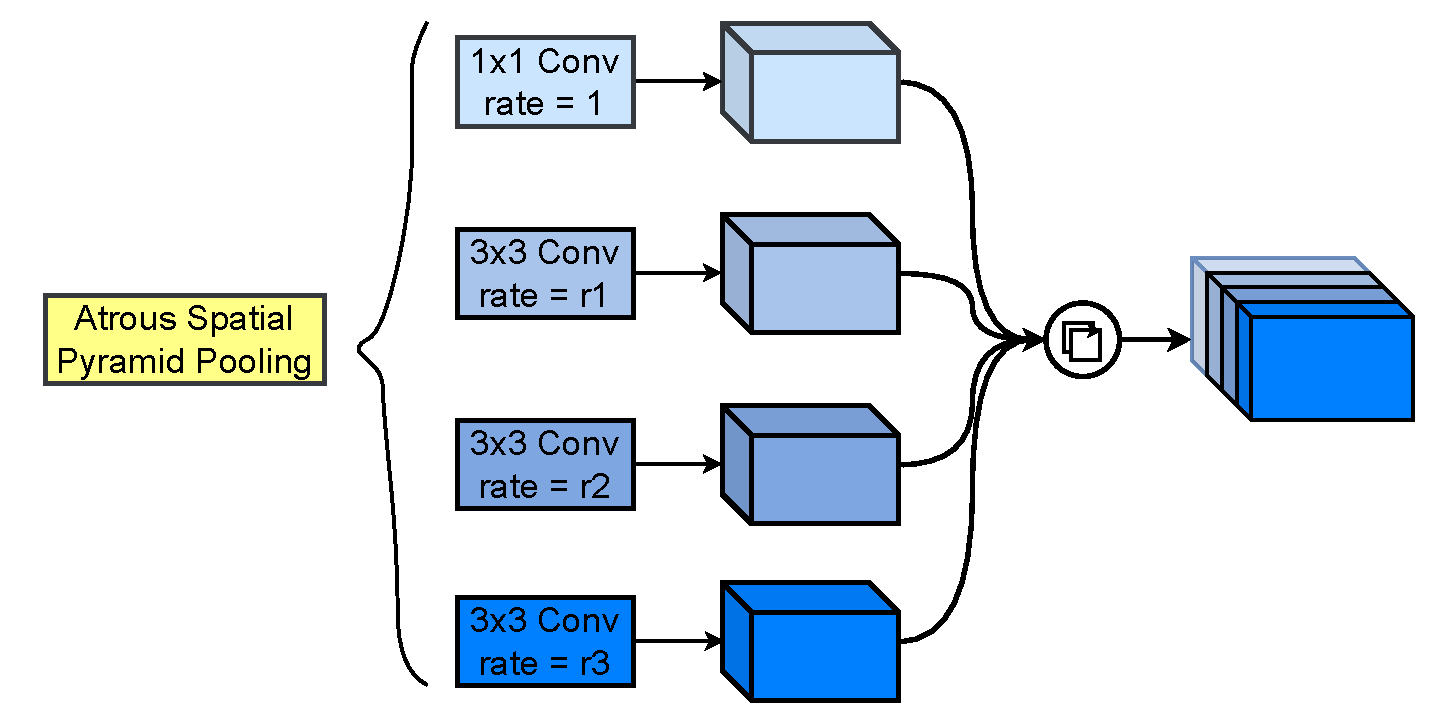
\includegraphics[width=0.45\textwidth]{img/Design-ASPP.pdf}
    \caption{The architecture of atrous spatial pyramid pooling module.}
    \label{fig3}
\end{figure}


On the other hand, ASPPs \cite{ChenAtrous} are employed within skip connection wires between encoder and decoder paths, they concatenate feature maps generated from the encoder path and pass them to the decoder path, they not only contain output feature maps in multiple receptive field sizes but also encode multiple scale informations, eventually boosting the performance of the network. In particular, as shown in Fig.~\ref{fig3}, the ASPP incorporates four parallel convolutional layers including a $\mathrm{1\times1}$ convolutional layer and three $\mathrm{3\times3}$ convolutional layers with different dilatation rates (i.e. $\mathrm{r_1, r_2, r_3}$). Consequently, the output of ASPP is synthesized by a depth-wise concatenation layer. Particularly, the output of ASPP module $\mathrm{F_{\text{ASPP}}}$ can be obtained as follows:
\begin{equation}
\begin{aligned}
    \mathrm{F}^\text{ASPP}_\text{out} =  \text{concat} (\text{conv}(1\times1,\mathrm{F}^\text{ASPP}_\text{in}), \\ 
     \mathrm{conv(3\times3,F^\text{ASPP}_\text{out},r_1)},\mathrm{conv(3 \times 3,F^\text{ASPP}_\text{out},r_2)}, \\ \mathrm{conv(3\times3,F^\text{ASPP}_\text{out},r_3))},
    \label{eq:ASPP}
\end{aligned}
\end{equation}
while $\mathrm{F}^\text{ASPP}_\text{in}$ is the input of ASPP, indexes ($\mathrm{r_1, r_2, r_3}$) represent for dilatation rates of three $\mathrm{3\times3}$ convolutional layers. Additionally, $\text{concat}$ denotes the depth-wise concatenation, and $\mathrm{conv}$ denotes the regular convolution. Regarding Fig.~\ref{fig4}, dilatation rates ($\mathrm{r_1, r_2, r_3}$) are defined as ($4, 8, 12$) at the first skip connection wire; ($3, 6, 9$) in the second skip connection wire; and ($2, 4, 8$) in the third skip connection wire, with with input of image sizes are $128\times128$; $64\times64$; and $32\times32$; respectively. These dilatation rates are defined to ensure that convolutional kernels effectively map to respective input image sizes, providing feature maps of multiple receptive field sizes to the decoder path.
\begin{figure}[!t]
    \centering
    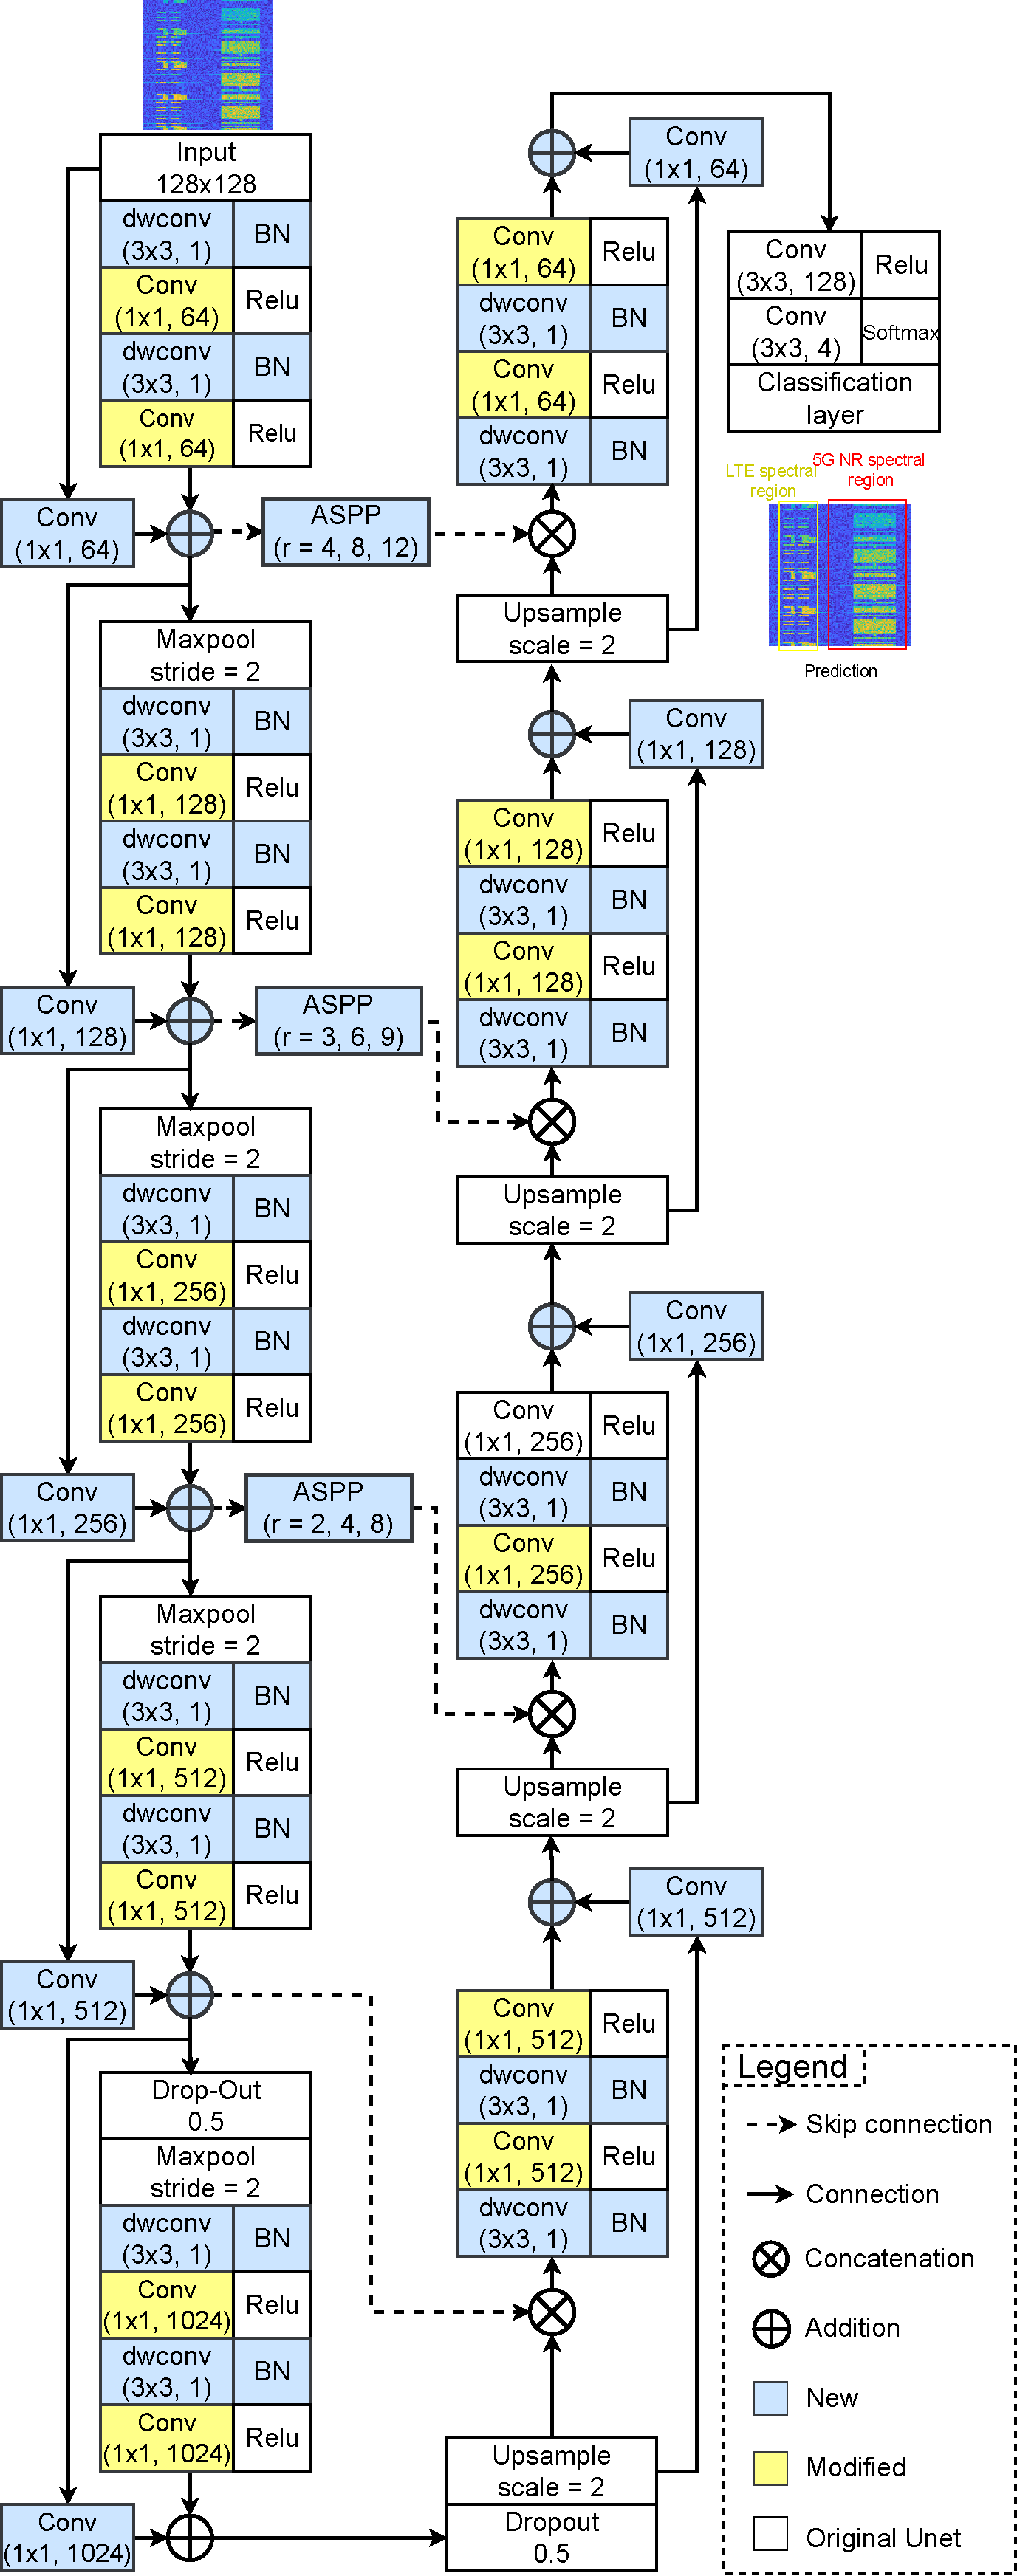
\includegraphics[width=0.45\textwidth]{img/Design-SpecSenseNet.pdf}
    \caption{The architecture of our proposed SpecSenseNet.}
    \label{fig4}
\end{figure}

Furthermore, inspiration from the architectural innovation of RRB as introduced in \cite{aghalari2021brain} and \cite{he2016deep}, we have revolutionized our network using RBB. Specifically, we have overhauled both encoder and decoder paths of our network by substituting the conventional U-Net convolution with RRB. In the SpecSenseNet architecture, the output of each RRB block is seamlessly integrated with a cascade of two DSCs and augmented by a residual path. This augmentation gains the richness of the features captured by our network and mitigates the vanishing gradient problem.
The operation of RRB can be described as follows:
\begin{equation}
\begin{aligned}
    \mathrm{F_\text{RRB}} = \mathrm{F}_\text{out}^\text{DSC} + \mathrm{conv(1\times1,\mathrm{F}_\text{in}^\text{DSC})},
    \label{eq:RRB}
\end{aligned}
\end{equation}
where $\mathrm{F_\text{RRB}}$ is the output of the RRB block, $\mathrm{F}_\text{out}^\text{DSC}$ represents for the output of DSC, and $\mathrm{F}_\text{in}^\text{DSC}$ is the input of the residual path connecting with $1\times1$ regular convolutional layer, respectively.






As shown in Table \ref{tab1}, when comparing network complexity between our design and other architectures, SpecSenseNet offers the minimal size of the network compared to the original U-Net architecture and its variants. Particularly, it decreases significantly the network's size to $7.8$M, reducing by $75.1\%$ and approximately $81\%$ comparing to U-Net and other variants (i.e. U-Netp, U-NetE, U-Netpp), respectively. Consequently, this enhancement contributes to improve training speed during the training phase. However, the number of layers in SpecSenseNet increases significantly as a result of replacing both depth-wise convolutional layers and point-wise convolutional layers with regular convolutional layers. Despite this modification, the network's performance during both the training and prediction phases is not significantly affected.

\begin{table}[!t]
\centering
\caption{Hardware resources and training options}
\label{tab2}
\begin{tabular}{c|c|c|c}
\hline
\multicolumn{2}{c|}{\textbf{Hardware Resources}} & \multicolumn{2}{c}{\textbf{Training Options}} \\ \hline
CPU & $3.0$GHz & No. epochs & $40$ \\ 
GPU & RTX $2080$ & Learning rate & $0.001$ \\
Memory & $16$GB & Learning rate schedule & $\mathtt{piecewise}$ \\ 
MatLab version & R$2023$ & Validation frequency & $1000$ \\
\hline
\multicolumn{4}{c}{\textbf{Dataset Information}} \\
\hline
\textbf{Category} & \textbf{No.Samples} & \textbf{Image size} & \textbf{SNR (dB)}\\
\hline
LTE         & $5,000$ & $128 \times 128$ & $[0, 30]$ \\
5G          & $5,000$ & $128 \times 128$ & $[0, 30]$ \\
5G and LTE  & $5,000$ & $128 \times 128$ & $[0, 30]$ \\
\hline
\end{tabular}
\end{table}

\section{Dataset, hardware resources, result and discussions}
\subsection{Dataset and training resources}

In this work, we consider realistic challenges such as cost and privacy. We use the 5G toolbox in MATLAB to generate synthetic 5G and LTE spectrums with three types: 5G only, LTE only, and overlapping 5G and LTE frames. Each type contains $5,000$ samples with an image size of $128\times128$ pixels. The signal-to-noise ratio (SNR) ranges from $0$ to $30$ dB. We split the dataset into $80\%$ for training, $10\%$ for validation, and $10\%$ for testing.
The training process is executed on a state-of-the-art computing system known for its high performance. The system features a powerful $3.00$ GHz central processing unit (CPU) and a cutting-edge NVIDIA RTX 2080 graphics processing unit (GPU). It also boasts a substantial $16$ GB of memory capacity.
During training, the learning rate is set to $0.001$ initially and adjusted using a piecewise learning rate schedule. The training process runs for $40$ epochs with validation occurring every $1,000$ iterations.
For more detailed information about the dataset and training resources, please refer to Table \ref{tab2}.


\subsection{Simulation and evaluation result}

\begin{table}[!t]
\centering
\setlength{\tabcolsep}{8pt}
\caption{Network Complexity Comparison}
\label{tab1}
\begin{tabular}{l|c|c}
\hline
\textbf{Network} & \textbf{No.Layers} & \textbf{No.Params} \\
\hline
U-Net \cite{ronneberger2015u} & $59$ & $31.3$M \\
U-Netp \cite{zhou2019unet++} & $101$ & $42.5$M  \\
U-NetE \cite{zhou2019unet++} & $101$ & $42.3$M \\
U-Netpp  \cite{zhou2019unet++} & $101$ & $43.5$M  \\
ConvNet  \cite{huynhthe2023intelligence} & $100$ & $20.6$M \\
Deeplabv3+ \cite{nguyen2023accurate} & $100$ & $20.6$M  \\
SpecSenseNet & $125$ & $7.8$M \\
\hline
\end{tabular}
\end{table}

We evaluate networks using four metrics: global accuracy, weighted intersection-over-union (IoU), and mean F1 score. These metrics are widely used to assess the performance of semantic segmentation models in predicting class labels for each pixel. In the semantic segmentation, global accuracy is the ratio of correctly classified pixels, regardless of class, to the total number of pixels. F1 score is the harmonic mean of precision and recall, providing a balanced view of both metrics, where precision refers to the proportion of predicted positive labels that are truly positive and recall measures the proportion of actual positive labels that are correctly identified by the model. Weighted IoU is a common metric in semantic segmentation, comparing the area of overlap between the predicted and ground truth segmentation masks. In Table \ref{tab3}, we report the results of our proposed deep model compared with some existing deep models the task of spectrum segmentation for intelligent spectrum sensing. 

\begin{table}[!t]
\centering
\caption{Simulation result comparison}
\label{tab3}
\begin{tabular}{l|c|c|c}
\hline
\textbf{Network}  & \textbf{G.Accuracy (\%)} & \textbf{W.IoU (\%)} & \textbf{M.BFScore (\%)} \\
\hline
U-Net  \cite{ronneberger2015u} & $98.22$   &  $96.53$ & $90.56$ \\
U-Netp  \cite{zhou2019unet++} & $98.07$   &  $96.24$ & $89.20$ \\
U-NetE  \cite{zhou2019unet++} & $97.84$   & $95.82$  & $88.05$ \\
U-Netpp \cite{zhou2019unet++}   & $97.98$   & $96.07$ & $88.89$ \\
ConvNet \cite{huynhthe2023intelligence}   & $39.69$  & $19.32$ & $15.61$ \\
Deeplabv3+ \cite{nguyen2023accurate}  & $46.26$  &  $33.87$ & $14.39$ \\
SpecSenseNet  & $97.23$  & $94.61$ & $87.32$  \\
\hline
\end{tabular}
\end{table}
\begin{figure}[!t]
    \centering
    \footnotesize
    \begin{tabular}{cccc}
        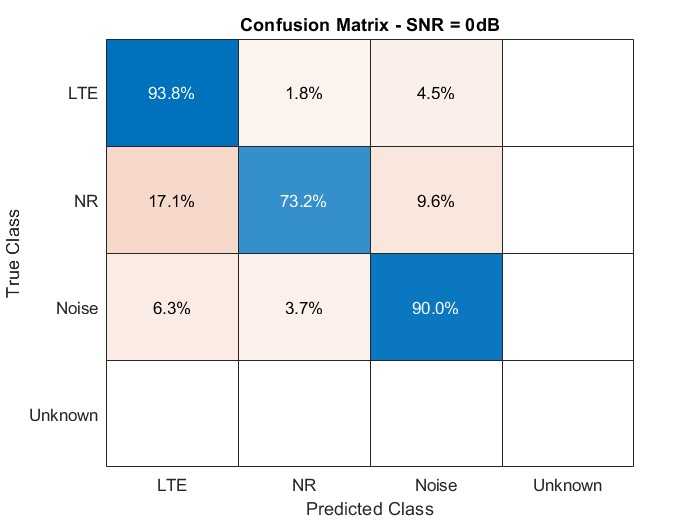
\includegraphics[width=0.25\textwidth]{img/confusion_matrix_0dB.jpg} & 
        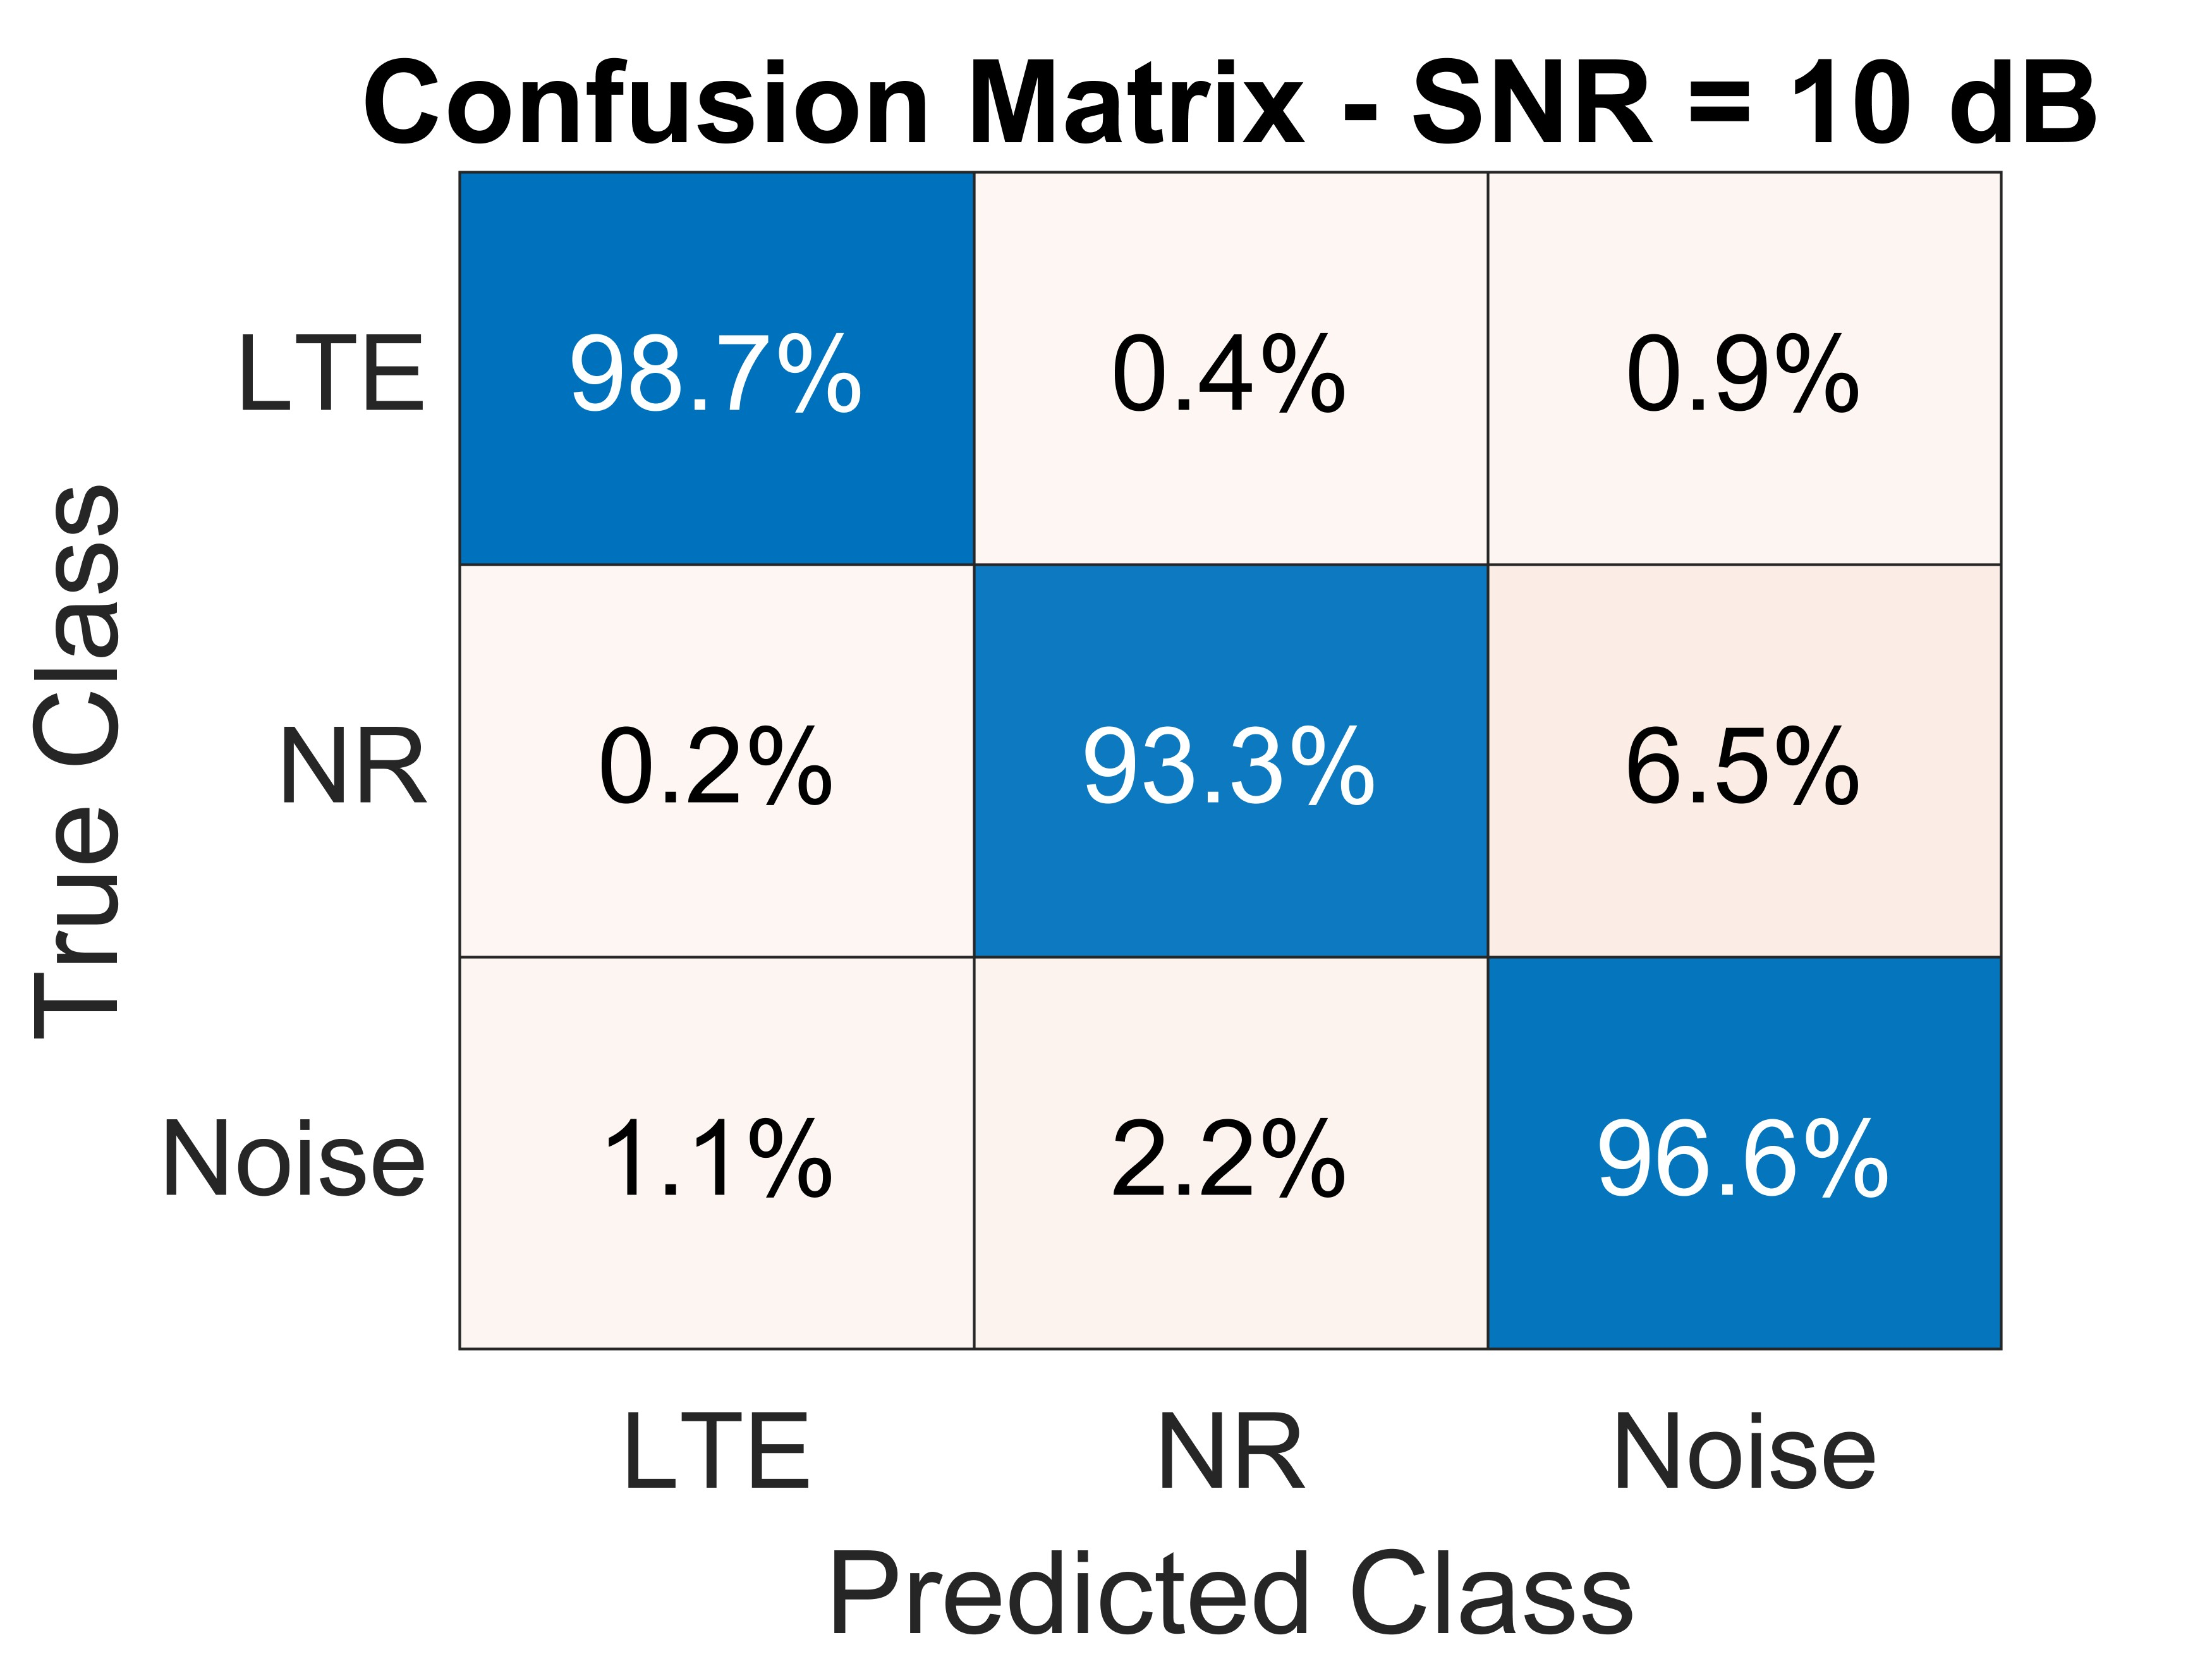
\includegraphics[width=0.25\textwidth]{img/confusion_matrix_10dB.jpg} & \\ (a) & (b) \\
        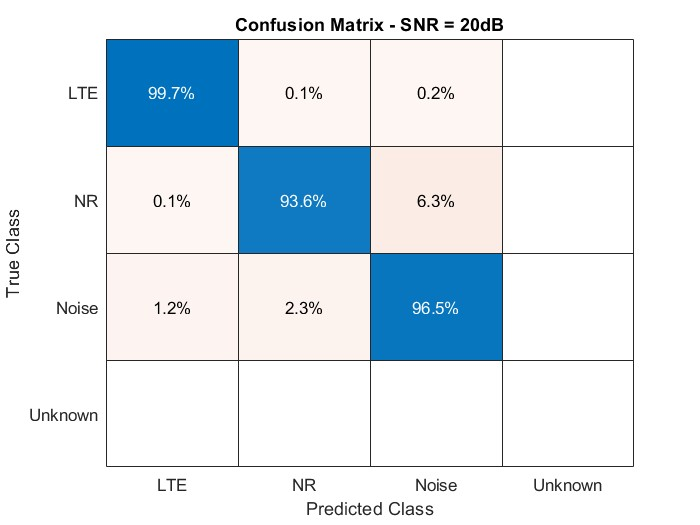
\includegraphics[width=0.25\textwidth]{img/confusion_matrix_20dB.jpg} & 
        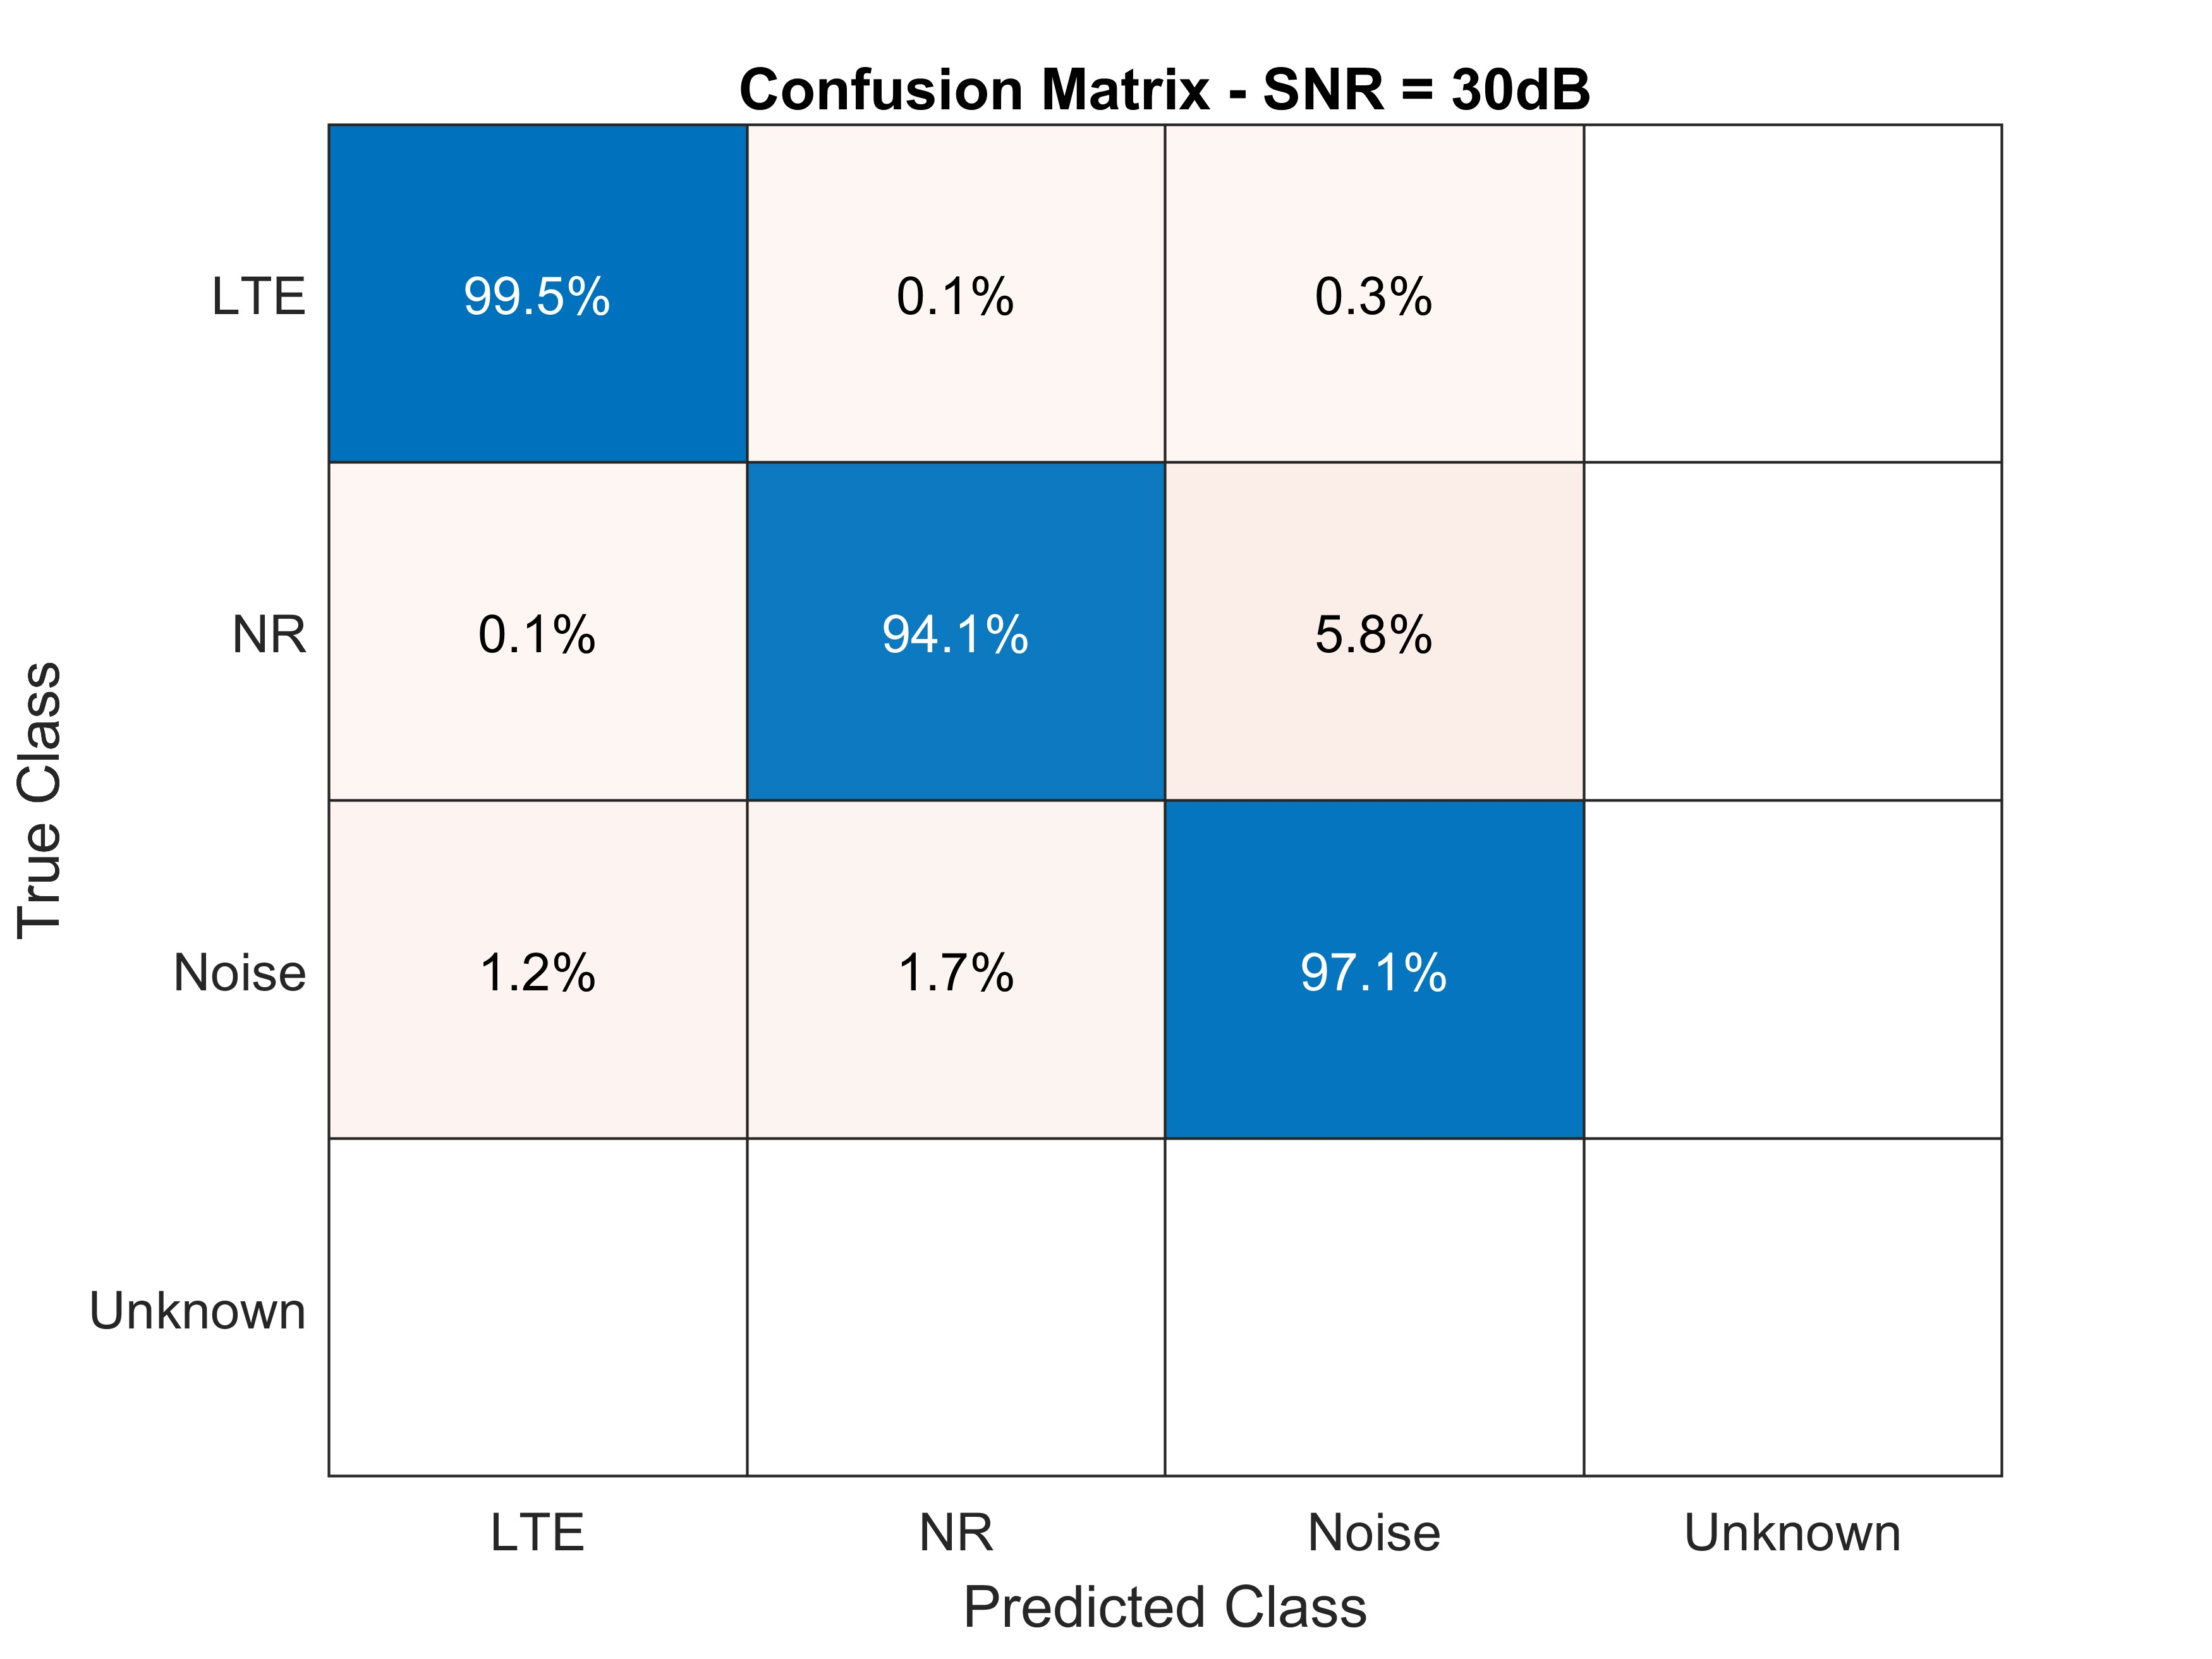
\includegraphics[width=0.25\textwidth]{img/confusion_matrix_30dB.jpg} & \\ (c) & (d)
    \end{tabular}
    \caption{Confusion matrix in different SNR levels: (a) $0$ dB, (b) $10$ dB, (c) $20$ dB, (d) $30$ dB}
    \label{fig5}
\end{figure}

\begin{figure}[!t]
    \centering
    \footnotesize
    \begin{tabular}{c}
        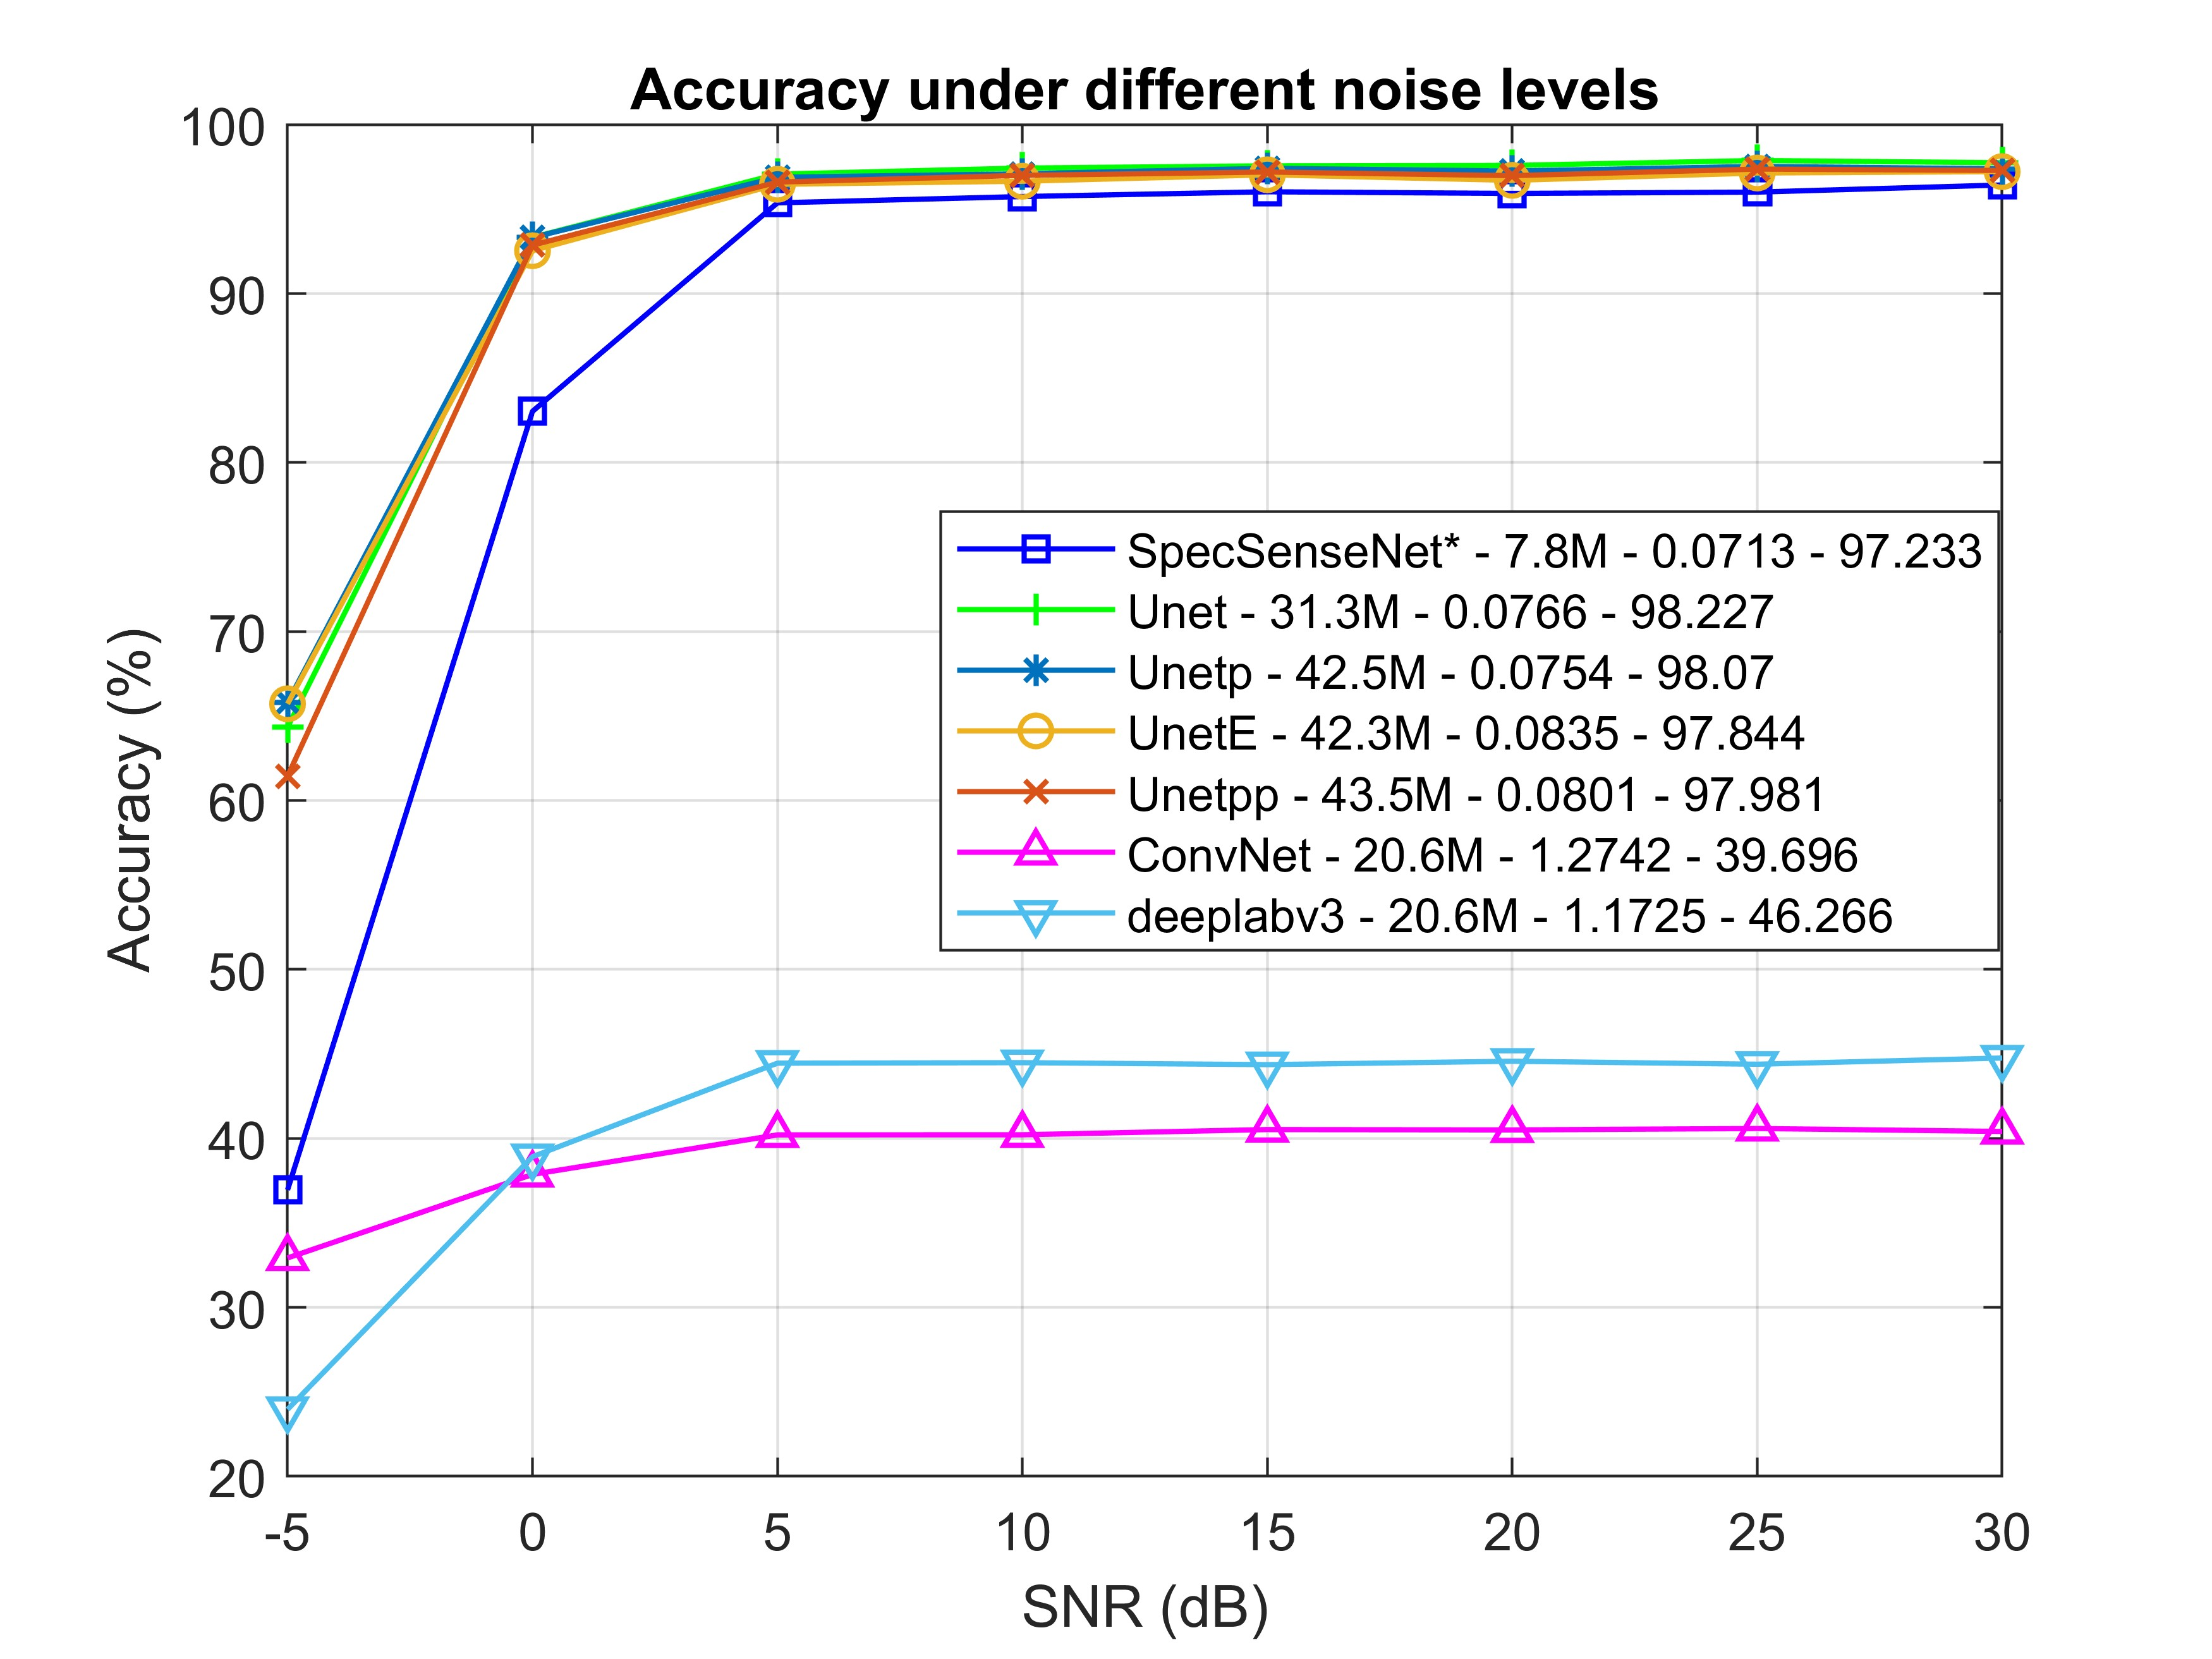
\includegraphics[width=0.5\textwidth]{img/accuracy_SNRs.jpg}
    \end{tabular}
    \caption{Accuracy evaluation under different noise levels}
    \label{fig6}
\end{figure}

\begin{figure}[!ht]
    \centering
    \footnotesize
    \begin{tabular}{ccc}
        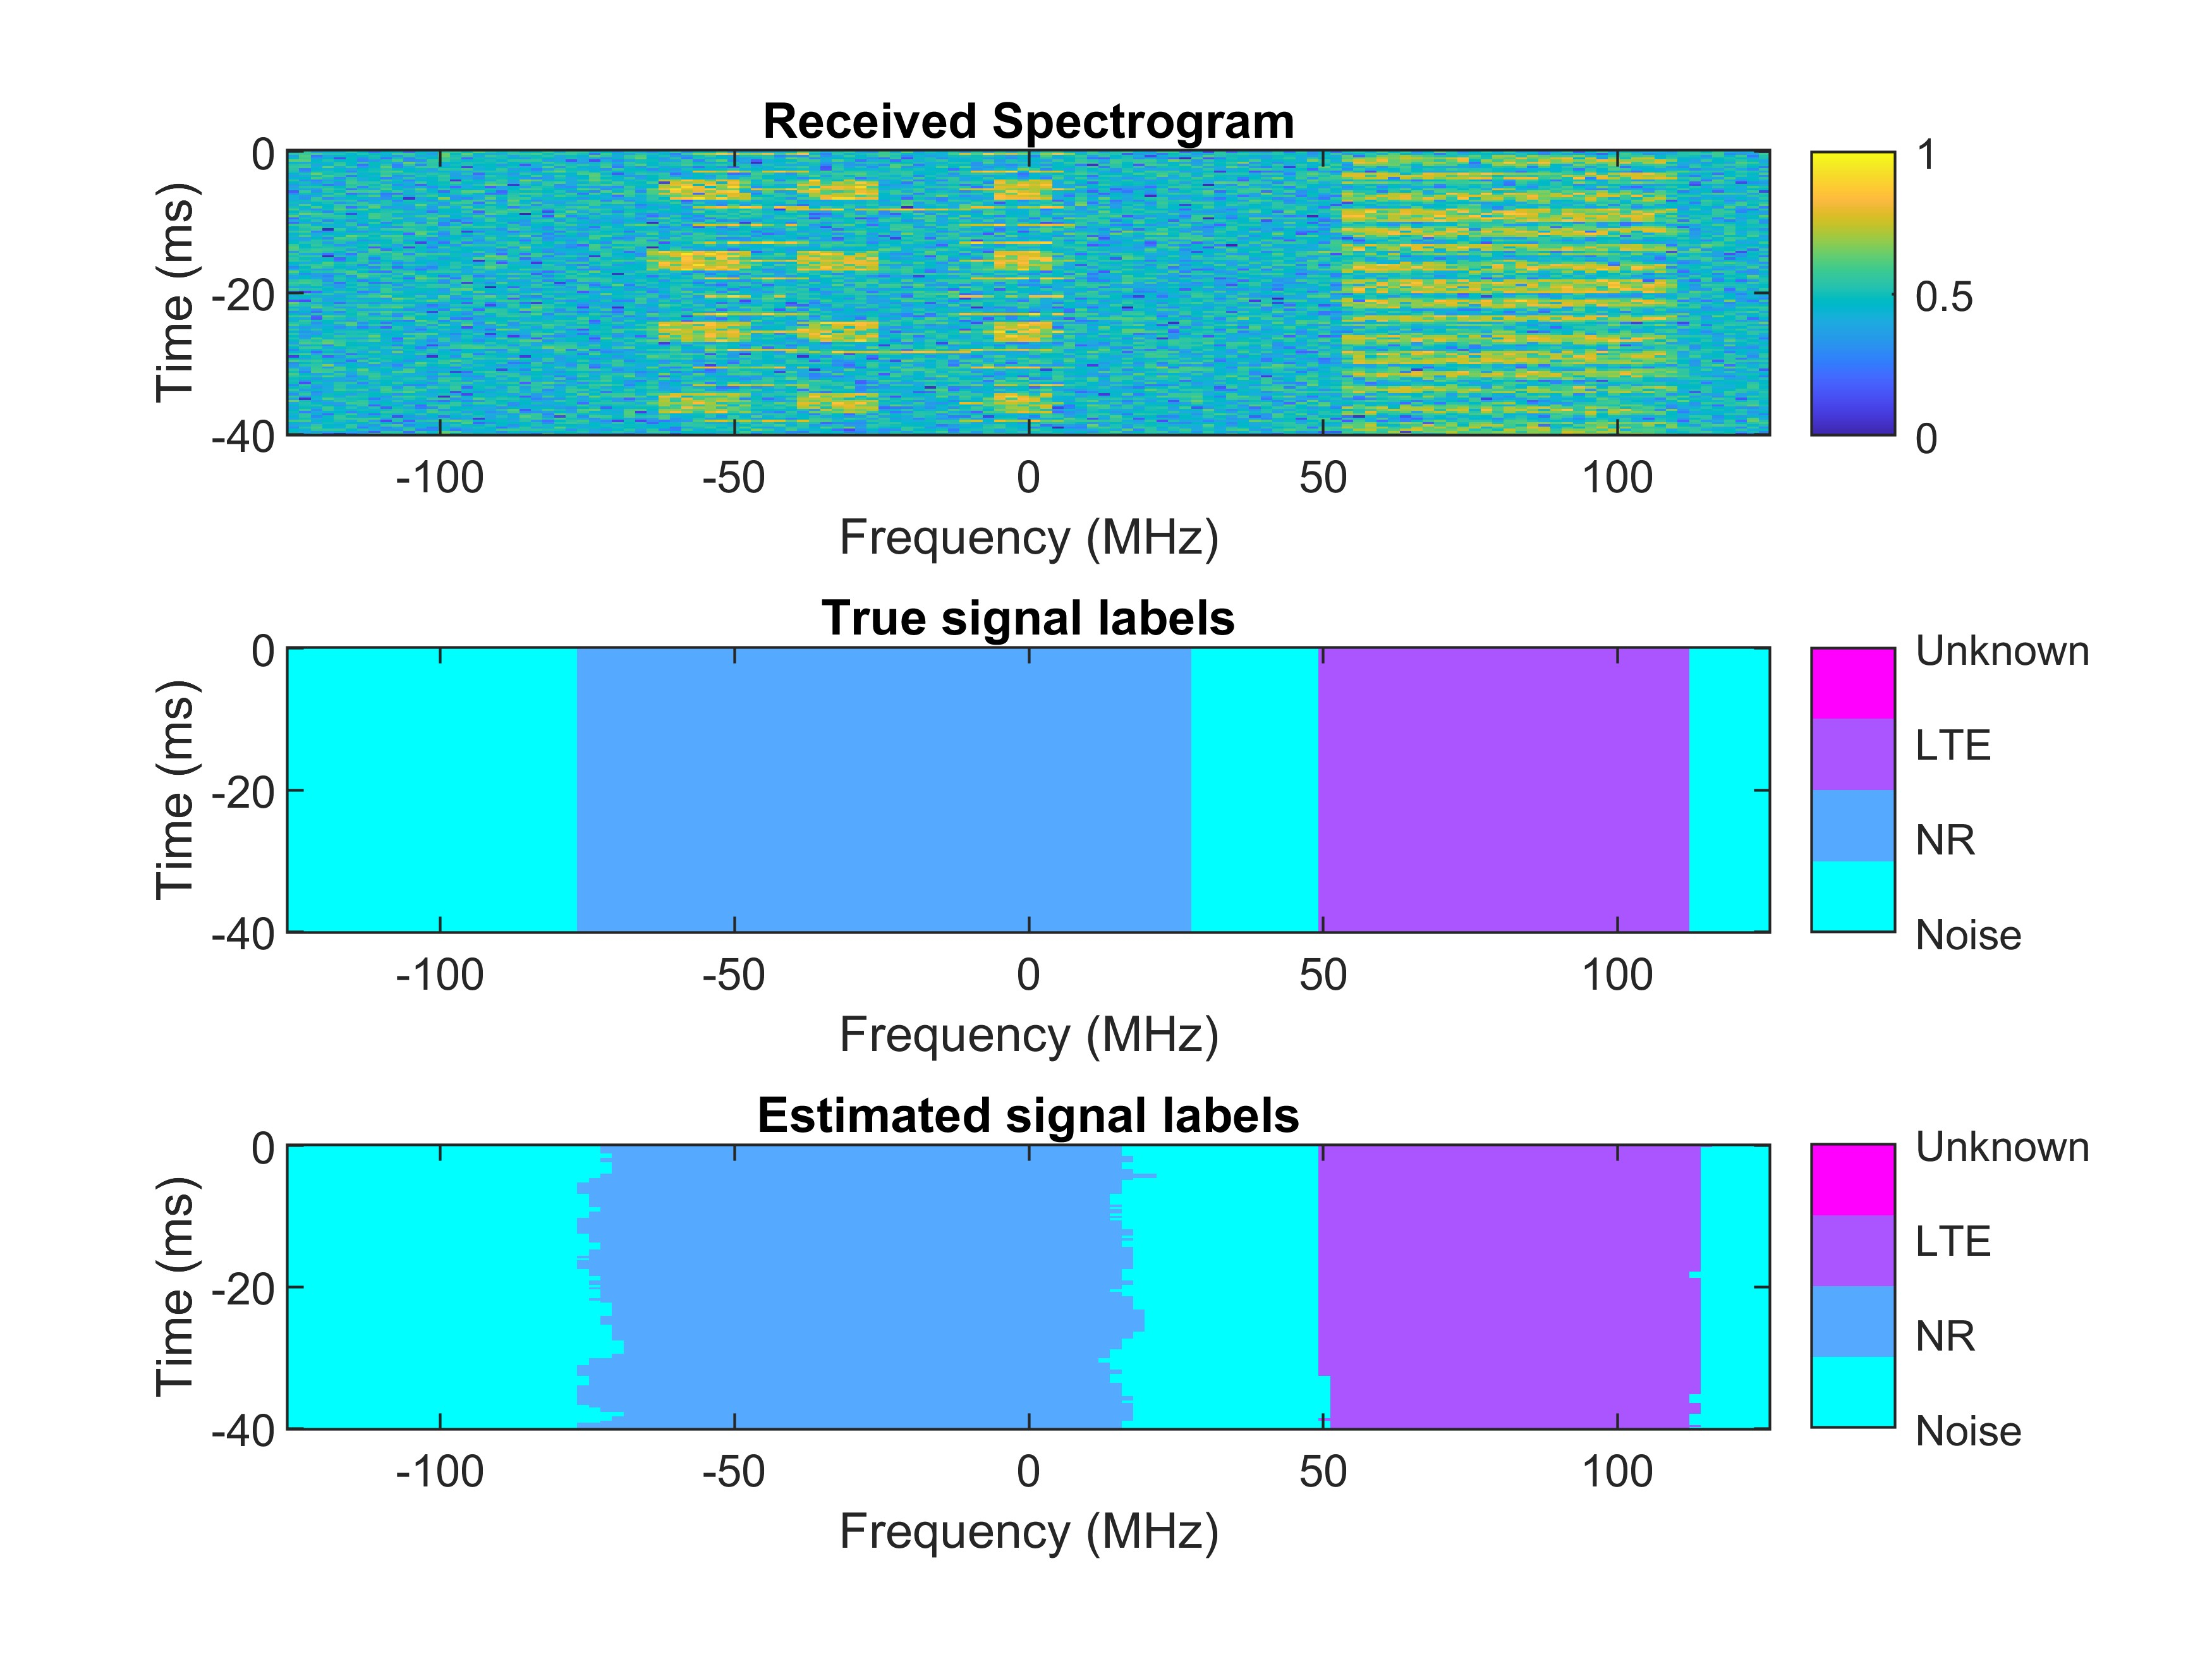
\includegraphics[width=0.45\textwidth]{img/Visualization_5dB.jpg} \\ (a)\\  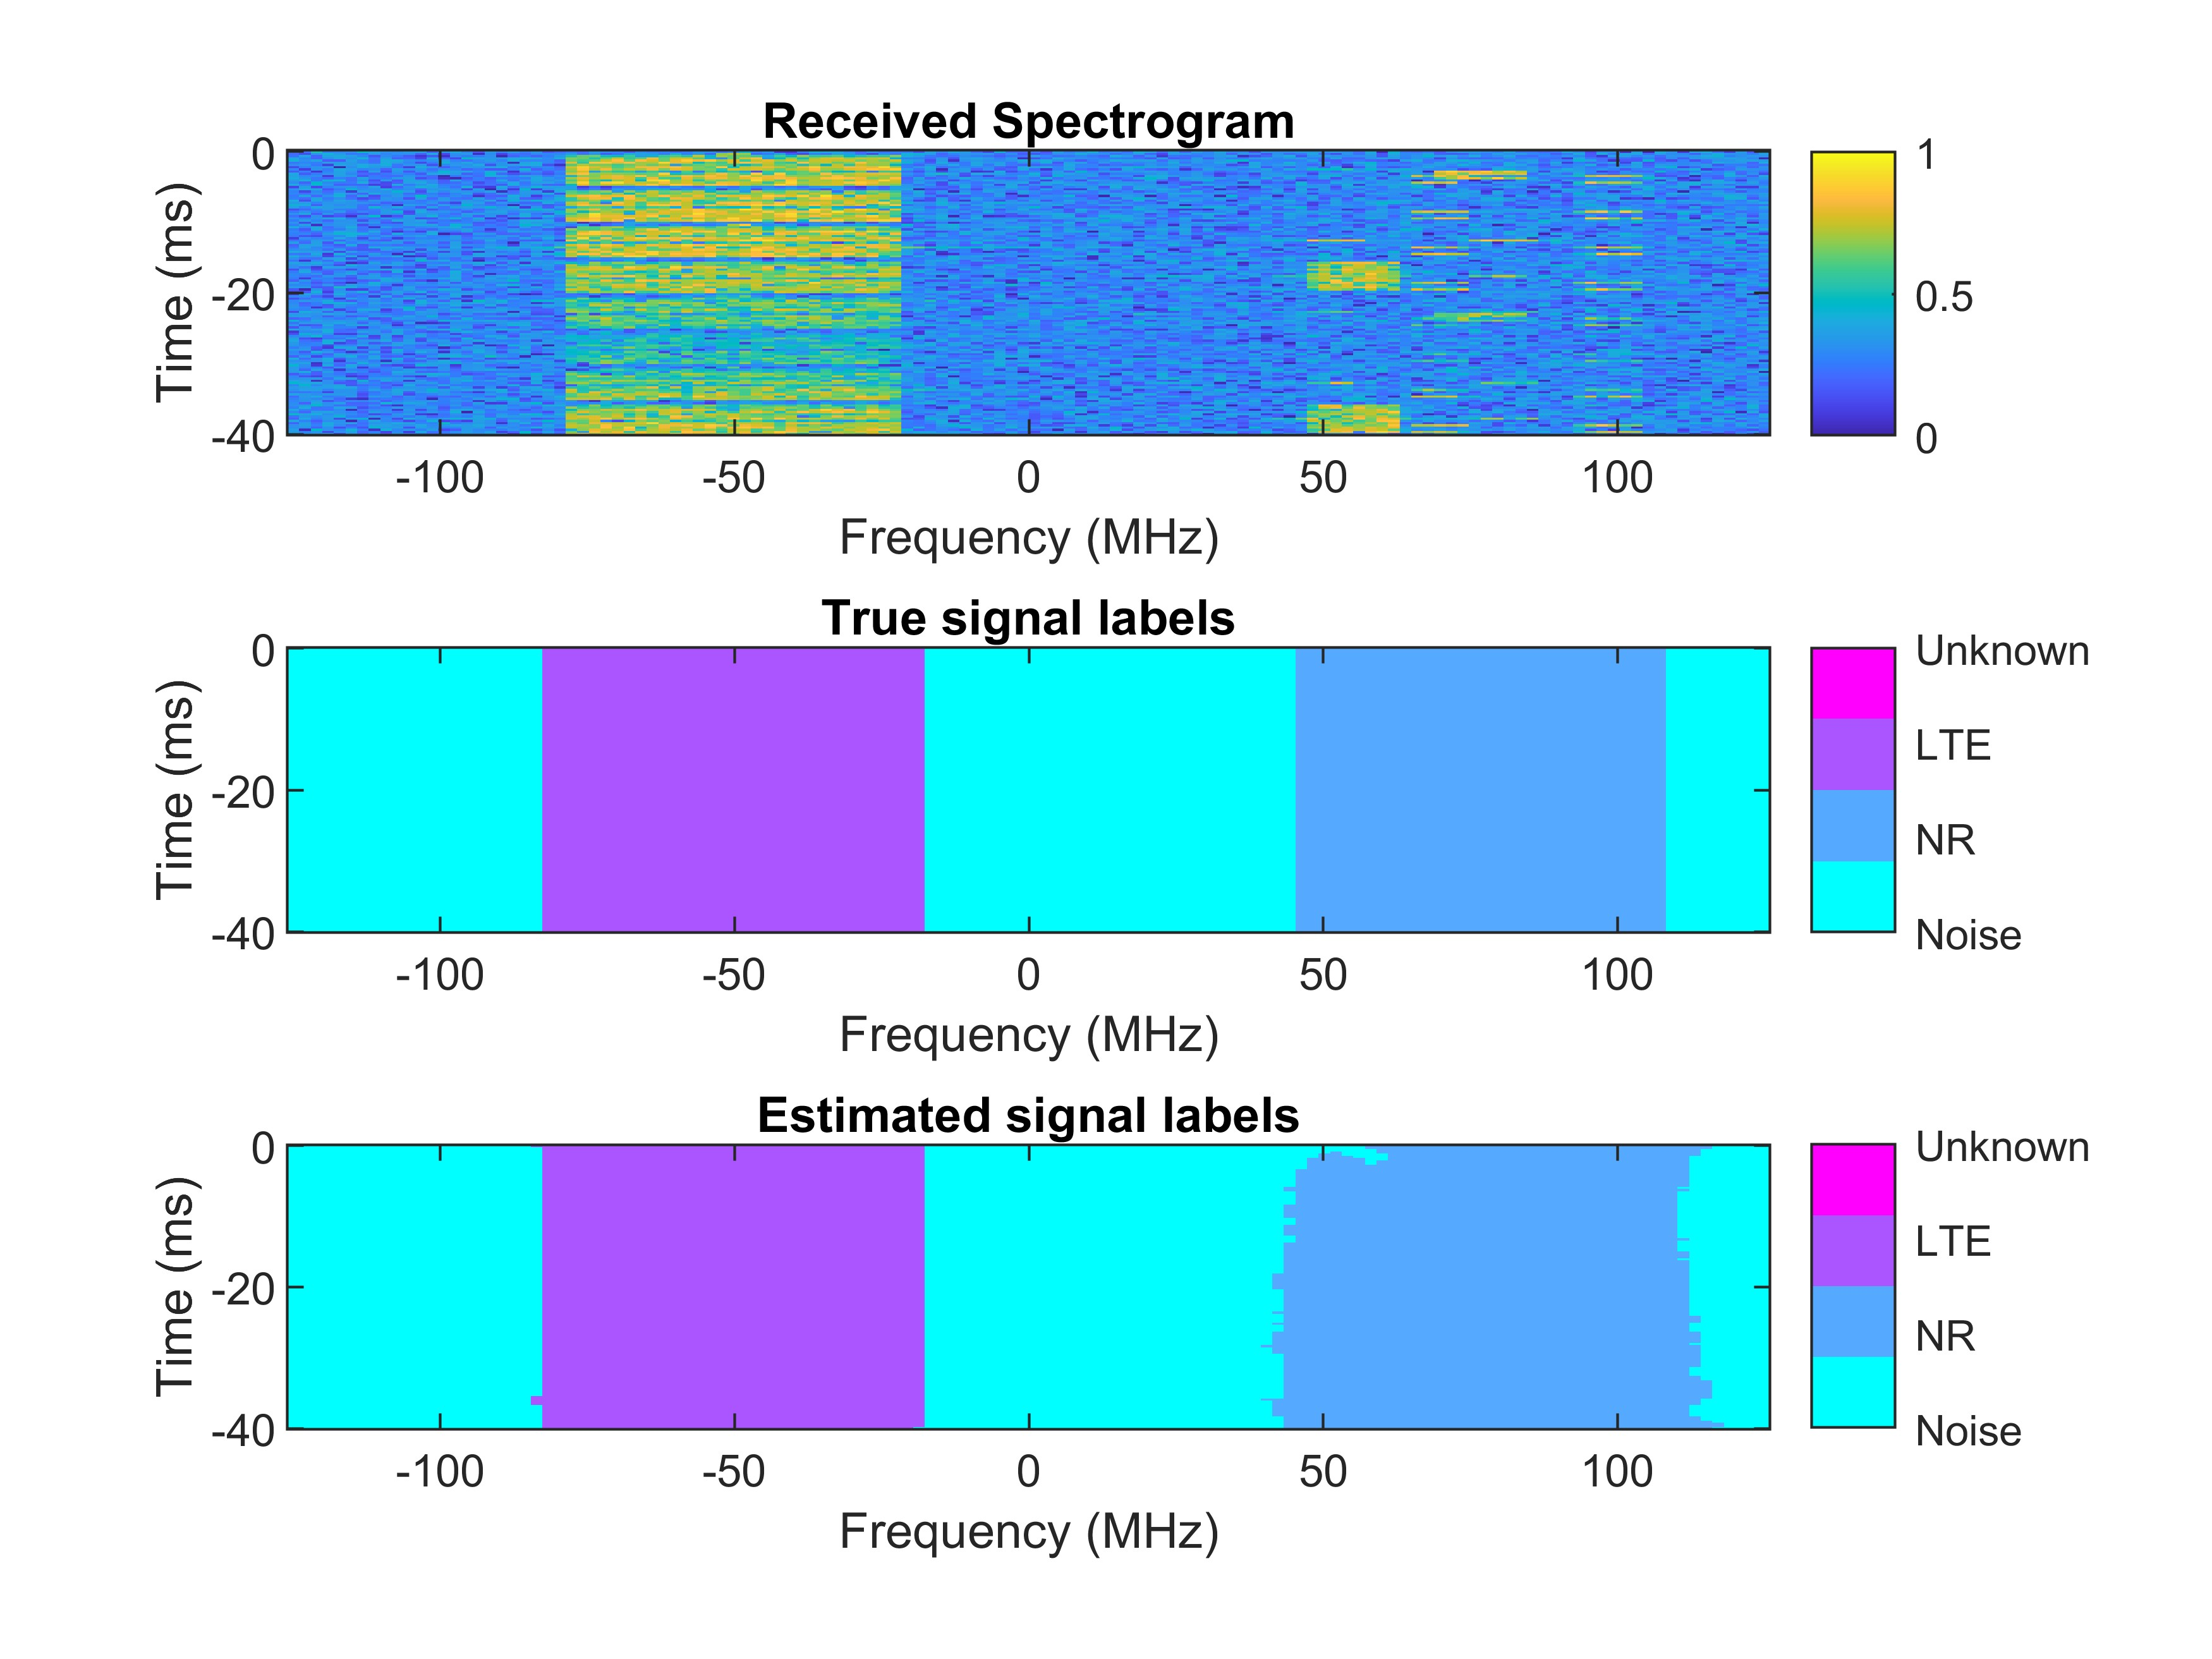
\includegraphics[width=0.45\textwidth]{img/Visualization_15dB.jpg} \\ (b)\\ 
        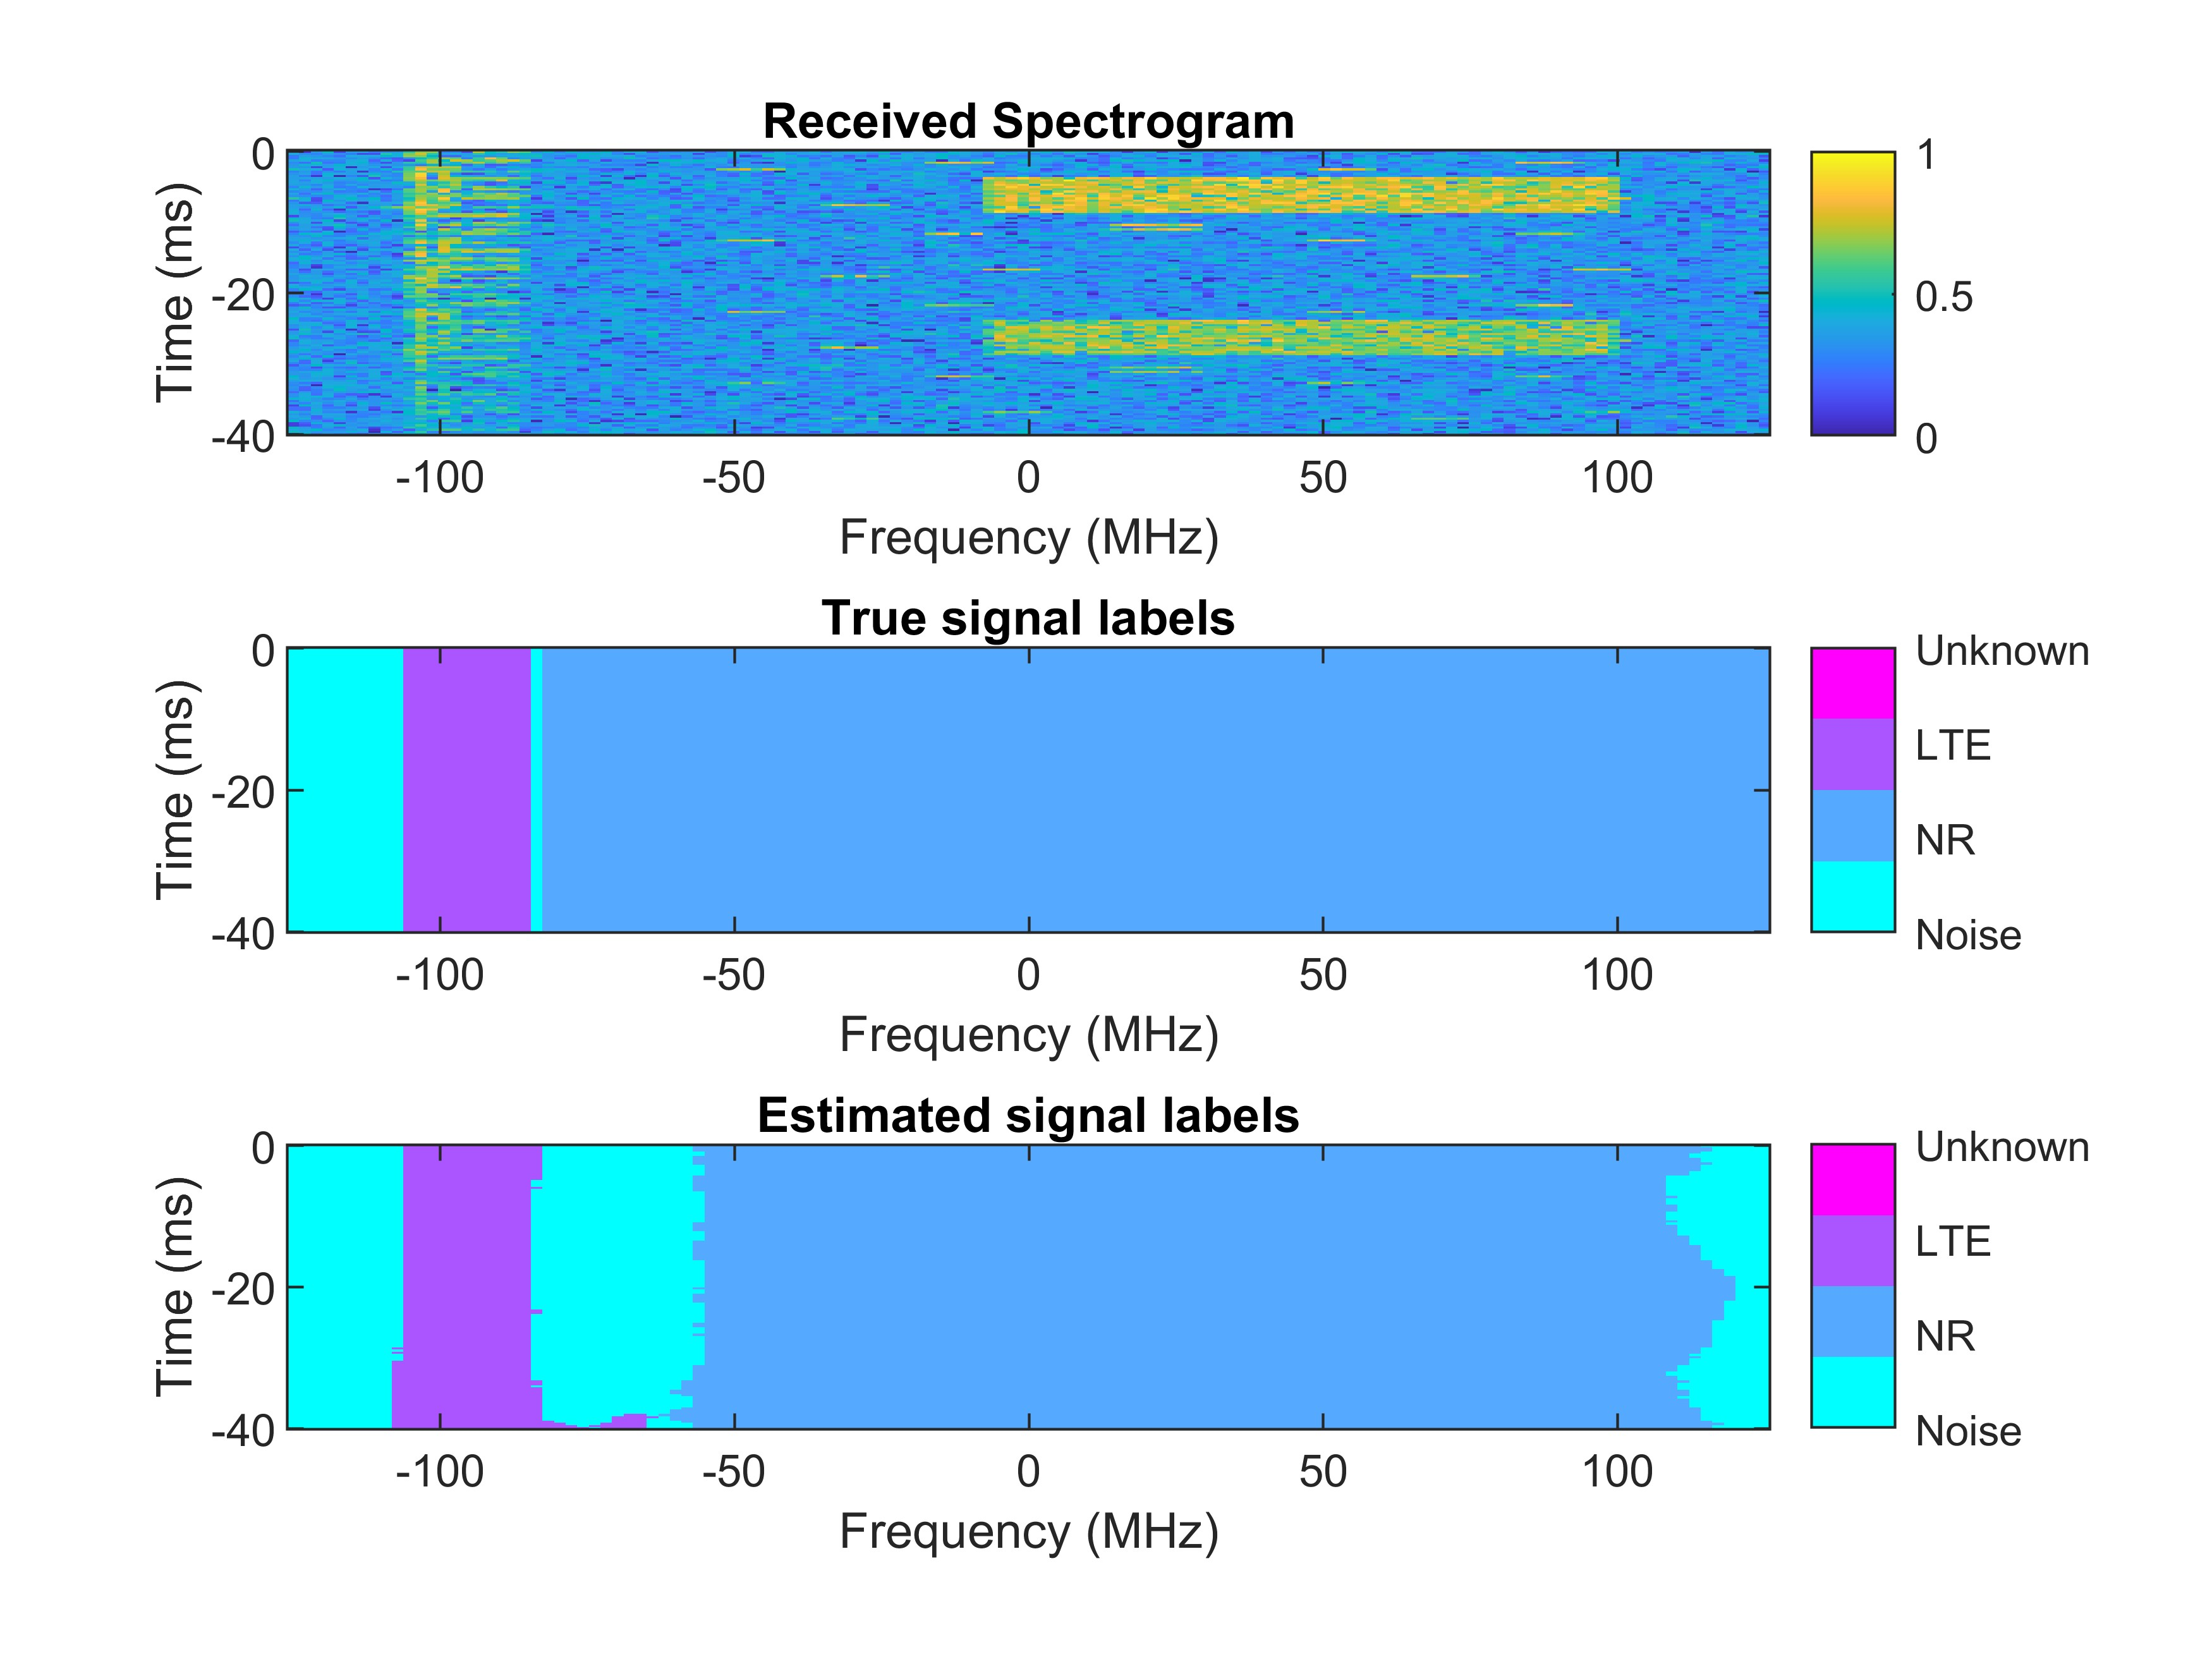
\includegraphics[width=0.45\textwidth]{img/Visualization_30dB.jpg} \\ (c)\\ 
    \end{tabular}
    \caption{Visualization of received spectrograms in various SNR levels: (a) $5$ dB, (b) $15$ dB, (c) $30$ dB}
    \label{fig7}
\end{figure}

According to Table~\ref{tab3}, SpecSenseNet achieves an impressive $97.22\%$ global accuracy, outperforming other models. ConvNet and Deeplabv3 have considerably lower accuracy, at $39.69\%$ and $46.26\%$, respectively. Our proposed network maintains consistently high accuracy and performance compared to U-Net-based architectures. It significantly reduces the network's size, leading to improved training and prediction speed. Notably, it achieves similar global accuracy to U-Net while reducing the number of parameters by $75.1\%$. Fig.~\ref{fig5} and~\ref{fig6} present confusion matrices generated during our network's evaluation with different levels of additive noise. They also show the training accuracy compared to other networks. Confusion matrices indicate successful outcome predictions across four classes in various SNR levels. As expected, the performance for estimating labels increases with higher SNR levels. Our network was trained on test samples spanning a wide range of SNR levels, from $0$ to $30$ dB. Fig.~\ref{fig6} demonstrates that our model achieves significant predictive accuracy across different SNR ranges, showing robust performance, especially at higher levels (above $5$ dB). In summary, these results demonstrate that SpecSenseNet significantly outperforms other models in semantic segmentation performance across all categories (5G NR, LTE, noise, and unknown).

Fig.~\ref{fig7} shows the segmentation results for several spectrogram samples at different SNR levels, such as$5$ dB, $15$ dB, and $30$ dB. This work specifically evaluated three overlapping 5G and LTE spectrogram samples at these SNR levels. The results demonstrate a clear improvement in segmentation accuracy across all SNR ranges. This includes the proportion of correctly predicted labels for 5G, LTE, noise, and unknown signals. At a $5$ dB SNR level (with moderate noise), the label predictions are generally accurate, although the estimated labels for 5G are not perfectly aligned with the true labels. However, there is a significant improvement in classification results at $15$ dB (lower noise). The gap between predicted and true labels becomes even smaller at $30$ dB (very low noise), achieving highly accurate predictions. With the segmentation results (a.k.a., the regions of interest of 5G and LTE signals on the spectrogram image), it enables communication systems to identify the time stamps and frequency ranges of signals automatically and accurately.
Additionally, the simulation results demonstrate that our network performs well and is suitable for real-world scenarios with varying noise levels.

\section{Conclusion}
In this paper, we introduced SpecSenseNet, a novel deep learning architecture based on U-Net. SpecSenseNet achieves impressive performance in spectrum sensing for 5G and LTE across various SNR levels.  Our work addresses the challenge of applying deep learning to spectrum sensing tasks. The proposed network leverages cutting-edge deep learning techniques to significantly reduce the number of trainable parameters compared to U-Net and other variants. This reduction in complexity enhances the efficiency of both training and prediction phases. In summary, simulations demonstrate that SpecSenseNet achieves robust classification for 5G and LTE spectrum sensing, even in the presence of high additive noise. This performance makes SpecSenseNet well-suited for real-world deployments.

\bibliographystyle{IEEEtran}
\bibliography{reference}
\end{document}


